\chapter{A Probabilistic Approach to Grasp Synthesis}
\label{chapter:gs}
Humans can grasp a wide variety of objects which differs from the shape, color, mass, etc. They can also well handle unknown objects which are presented to them for the first time. In order to have a general purpose robot which can help people in the unstructured human environment, grasping unfamiliar items is a must-have skill to achieve this goal. In this chapter, we consider this aspect of the grasping problem and provide methods on how this problem can be solved. 

\section{Introduction}
Robotic grasping is a quite old problem which has been studied over 20 years. Although the speed and resource of computers increase dramatically, the grasping capability of robots is still far behind the human. The main reason is that there is a big gap of skills between humans and robots. These skills, which are essential for the grasping tasks, include cognitive level, the ability of abstraction and manipulation experience. In the recent year, with the emergence of low-cost sensors, high-speed graphical card, some progress has been made from theoretical grasp quality analysis to real grasping problems. Solving the problem of unknown object grasping becomes one of the frequently addressed problems in the research community because it is one of the necessary steps for robots toward human-level intelligence of manipulation.

The primary challenge of solving grasping unknown objects can be summarized in two aspects. The first one is associated with a wide variety of objects existed in the world. The variety of objects exists  in their appearance, shape, geometry, dynamics, etc. To model them individually is not a solution. How a robot can handle this variety is a big challenge. On the other hand, robots also have a limited sensing capability. The measurement from a sensor is never perfect. For example, the sensor data from an RGB-D camera contains not only the errors caused by noise but also errors caused by reflective or transparent object surface. To manage the uncertainty of sensing is another challenge. 
  
In recent years, methods which address this problem shifts from the traditional way of analyzing grasp stability to a data-driven / sensor-guided fashion. The  sensors which are often used for this task are RGB or RGB-D cameras. Former provides only image data while latter provides additional depth information of the environment. The RGB data provides the appearance information while the depth data encodes the shape property of objects. For the methods which only use an RGB camera as the primary sensor, they can only work in a given environment where the height of  grasping can be determined by the heuristic. For those who use an RGB-D camera as the primary sensor, correctly handling the uncertainty of depth measurement is a challenge. 

Previous works which address the problem can be categorized into two classes. The methods in the first class typically use a learning based method~(\cite{Kroemer2010},\cite{Tegin2009},\cite{Stulp2011}). These methods infer the grasp configuration directly from the sensor data. Supervised learning is used to build a model for grasp evaluation. A large training set is normally required to build the grasp evaluation model. The methods in another class use a shape based approach~(\cite{Miller2003},\cite{Przybylski2011},\cite{Goldfeder2007}), they first infer the shape of objects from the sensor data. Then, the grasp configurations are searched based on the shape estimate. Our method can be categorized into the second class, as we believe the form of an object provides the most clues on whether a grasp configuration may succeed or not. 

Different from previous work, we propose a probabilistic approach to address the grasp synthesis problem. Our approach contains two building blocks for finding a good grasp configuration. In the first building block, we solve the problem of evaluation of a given grasp. To do this, we need a model to represent the shape of an object and a model of evaluating a grasp. As we have suggested that shape contains the most information for grasping, it is most suitable to represent an object by its shape. For this purpose, we propose an object model called
 probabilistic signed distance function (p-SDF) to represent unknown object surface. p-SDF models measurement uncertainty explicitly and allows measurement
 from multiple sensors to be fused in real time. To evaluate a given grasp configuration, we propose four heuristics to perform the calculation. Each heuristics models one aspect which can influence force closure. The heuristics are combined in a weighted fashion to obtain the probability of force closure . 

In the second building block, we address the problem of finding the optimal grasp by searching the configuration space. For this purpose, we propose a generic gripper parametrization method which reduces the grasp configuration space. This is done by first organizing the joints from the same gripper finger into a collective group, and using a single parameter to control the movement of the joints belonging to the same finger. In this way, the grasp configuration space can be searched more efficiently. Finally, a  two-stage method based on simulated annealing is proposed to find the optimal grasp configuration. We validate the whole approach using real world challenging objects in our experiment. The result shows that our method can handle a variety of objects in a table-top environment. 
\section{Related work}
Up to 2010, most previous works addressed this problem by assessing the grasp stability with grasp quality metrics~\cite{Ferrari1992}. However, this approach is not scalable to the variety of real world objects, as grasp quality metrics mostly assumes an existing 3D object model. Later, the emergence of low-cost RGB-D sensors such as Kinect opened a new opportunity to study grasp synthesis in a data-driven fashion. Bohg et al.~\cite{Bohg2014} took a comprehensive survey on data-driven grasp synthesis. These approaches exploit 2-D vision~\cite{Glover2008}, RGB-D~\cite{Berenson2007} or multi-modal information~\cite{Bohg2010} to generate grasps for real world objects. In this section, we provide a review on methods of grasp synthesis, and focus on those which consider the following two aspects, how to handle the uncertainty, and pros/cons of learning based methods. 

\subsection{Methods considering pose uncertainty}
Handling uncertainty is considered as one of the most difficult problems, not only in grasping but also in many other fields of robotics. In (\cite{Goldberg1990},\cite{Hsiao2011},\cite{Chen2015}), grasping is modeled within a probabilistic framework to take variance in shape and pose into account. The methods can choose the most robust grasp configuration in spite of uncertainties in the perception and control. Pose and shape uncertainty are two common sources that make grasping difficult. Pose uncertainty can be reduced by exploiting finger tip tactile sensing \cite{Dang2014}\cite{Felip2009}\cite{Dragiev2013},  planning pre-grasp \cite{Dogar2011}\cite{Brost1988} or post-grasp \cite{Paolini2014} strategies. Some other approaches (\cite{Weisz2012},\cite{Kim2013}) proposed new grasp quality metrics that evaluates a grasp with pose uncertainty. Approaches considering pose uncertainty always assume an available object model and a perceptual system which predicts the pose uncertainty. 
\begin{figure}[!htbp]
    \centering
    \begin{subfigure}[b]{0.48\textwidth}
        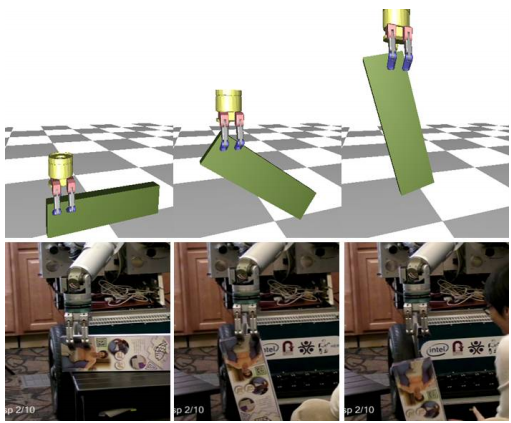
\includegraphics[width=\textwidth]{kimposeuncertainty.png}
        \caption{}
    \end{subfigure}
    \begin{subfigure}[b]{0.48\textwidth}
        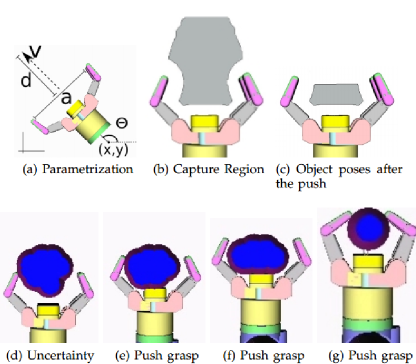
\includegraphics[width=\textwidth]{push_grasp.png}
        \caption{}
    \end{subfigure}
    \caption{(a) A grasp synthesis method proposed by \cite{Kim2013}. They consider the pose uncertainty by  simulating object dynamics. More stable and natural grasp sets can be generated. (b) A method using pre-grasp manipulation to address the pose uncertainty~\cite{Dogar2011}. They propose a planning framework which allows a robot to interact with objects by a library of actions such as push, slide or sweep operations. The pose uncertainty is addressed by the funneling effect of pushing.}\label{fig:rw_pose_uncertainty}
\end{figure}

\subsection{Methods considering shape uncertainty}
By contrast, approaches considering shape uncertainty do not require such information. Some methods simplify the problem to a two-dimensional planner setting. In \cite{Christopoulos2007}, Christopoulos et al. proposed how to handle shape and contact location uncertainty of a 2D object contour segmented from an image. Kehoe et al. \cite{Kehoe2012} proposed an approach to generate zero-slip push grasps based on object shape perturbations. For the methods which explicitly consider the shape uncertainty, the choice of object representation is a problem. Gaussian process (GP)\cite{rasmussen2006gaussian} is a powerful tool for modelling uncertainty. In \cite{Mahler2015}, \cite{Li2016} and \cite{Dragiev2011}, Gaussian process implicit surfaces (GPIS) \cite{Williams2007} are used to represent  shape uncertainty. Mahler et al. exploited GP in two dimension points, whereas Li et al. used GP to represent 3-D objects. However, there are some remarkable drawbacks in GP-based representation. The first drawback is the heuristic choice of training points. GPIS is obtained by a given set of points which represent the object surface, the space outside the object and the space inside the object. While surface points can be obtained from sensor measurement, points inside and outside the object are chosen heuristically. The shape uncertainty is dependent on this heuristics. The distance between two neighboring points determines the shape uncertainty. The real measurement uncertainty of the sensors can not be considered. The second drawback is related to computational complexity. The complexity for training a GP is $o(N^3)$, where $N$ is the number of points used for estimating the shape. Thus, GPIS does not scale to a large number of points. To find a trade-off between accuracy and computation complexity, these approaches filter out a large proportion of points obtained from sensor data, thus reduce the accuracy of the shape. In this work, we also use the implicit surface to represent objects, however, instead of using GP to estimate shapes, we use our approach described in \cite{Dietrich2016} to determine the object shape. This method is an extension of \cite{newcombe2011kinectfusion} for modeling shape uncertainty. We use all the measurement points and integrate them into a consistent model so that the resulting object shape is as accurate as possible. Besides, we also model the error characteristics of the sensors so that uncertainties expressed in the model explicitly reflect the characteristics of the used sensors. 
\begin{figure}[!htbp]
\centering
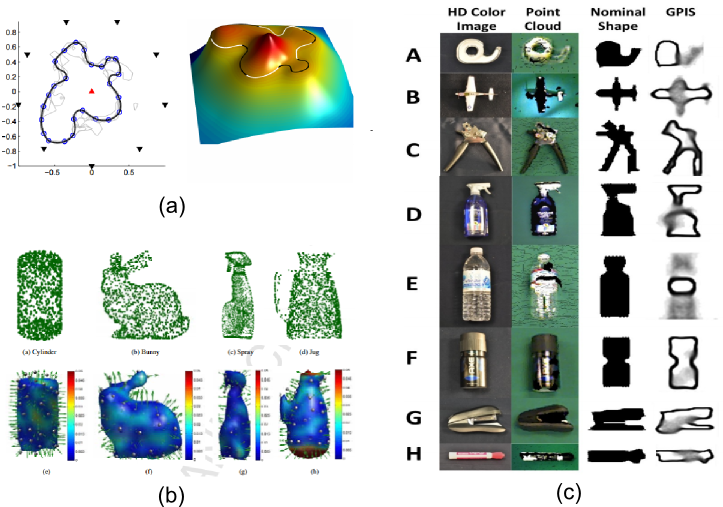
\includegraphics[width=0.9\linewidth]{relatedgpis.png}
\captionsetup{justification=raggedright}
\caption{(a) A method of representing object shape by Gaussian process implicit surface (GPIS) \cite{Williams2007}. (b) A method for grasp synthesis considering shape uncertainty in 3D. They use GPIS to represent shape uncertainty of objects. The points for training the shape model is obtained from synthetic data \cite{Li2016}. (c) A method for grasp synthesis considering shape uncertainty in 2D \cite{Mahler2015}. The points for training the shape model is obtained from real sensor.} 
\label{fig:rw_gpis}       % Give a unique label
\end{figure} 
\subsection{Methods using learning based approach}
Several learning based methods are proposed to solve the problem. Learning can be conducted either from human demonstration~(\cite{Herzog2014},\cite{ekvall2007learning},\cite{Romero2009}), from labeled database~\cite{Lenz2015} or from robot's own experience~(\cite{Pinto2015},\cite{Levine2016}). 
\begin{figure}[!htbp]
\centering
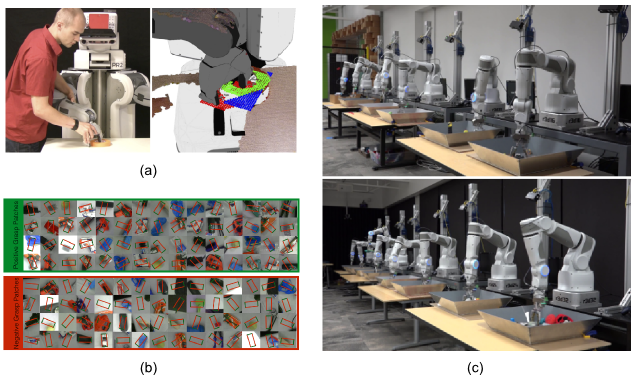
\includegraphics[width=0.9\linewidth]{rw_learning.png}
\captionsetup{justification=raggedright}
\caption{Learning based methods require a training set which include objects and associated grasps examples. Different methods can be used to acquire the training set. (a) Using human demonstration~\cite{Herzog2014} (b) Execute random grasps with a single robot to acquire positive and negative grasp examples.~\cite{Pinto2015} (c) Using a robot farm to acquire the training set.~\cite{Levine2016}} 
\label{fig:rw_deeplearning}       % Give a unique label
\end{figure}  
There are two classes of methods to address this problem. The first class is a feature-based approach. These approaches try to find specific features such as shape features, multi-modal features from the input data. These features are used to access the feasibility of a grasp. Eppner et al.~\cite{Eppner2013} demonstrated one method in which they tried to match the shape of objects to the grasp type. A similar idea is also described in~\cite{Huebner2008}. Herzog et al.~\cite{Herzog2014} proposed to select grasps based on shape template features. Jiang et el.~\cite{Jiang2011} extracted a rectangular feature to detect grasp configuration. All these approaches require some degree of discretization of the input data, which removes the details of the surface information. For tasks which require precision grasp, these methods are not suited.

Fischinger et al.~(\cite{Fischinger2012},\cite{Fischinger2015}) proposed height accumulated features to handle the problem of grasping unknown objects in clutter in a table-top scenario. The process of finding a grasp is illustrated in Fig.~\ref{fig:rw_haf}. An RGB-D sensor first captures the target scene. The obtained point cloud is then discretized into a height grid. A set of features is extracted from the height grid. The feature along with a candidate grasp is then classified using a set of pre-designed features to determine if the candidate grasp is feasible or not. Multiple candidates are tested and the method returns the grasp with the best score for final execution. Later, we use this method as the baseline for comparison. 
\begin{figure}[!htbp]
\centering
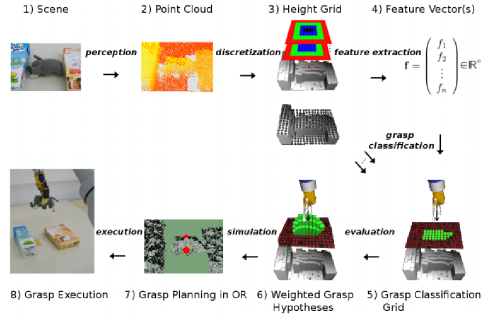
\includegraphics[width=0.9\linewidth]{rw_haf.png}
\captionsetup{justification=raggedright}
\caption{ A method using hand-crafted feature for grasp classification proposed by \cite{Fischinger2015}. The method discretizes input point cloud into height map. Features are extracted from height map for grasp classification. The best grasp is calculated by weighted grasp hypotheses and realized in a grasp planning simulator. Later, we use this method as baseline for comparison.} 
\label{fig:rw_haf}       % Give a unique label
\end{figure} 

The second class of approaches exploits machine learning methods to transfer the capability of  grasping known objects to unknown objects. It has been noticed recently, the representational power of hand-crafted features is not always sufficient. It might be better to let the system learn them itself. For this purpose, some researchers apply deep learning to solve this problem. Lenz et al.~\cite{Lenz2015} demonstrated how deep learning can find features automatically from multi-modal information. Redmon et al.~\cite{Redmon2015} optimized the performance of grasp detection by a convolutional neural network using the same dataset as Lenz did. In~\cite{Pinto2015}, Pinto et al. demonstrated that by gathering the grasping dataset with a real robot over 700 hours, the same approach achieves higher accuracy. Learning can also be exploited to approximate the probability density of contact models. Kopicki et al.~\cite{Kopicki2014} proposed this concept to generalize dexterous grasp from known objects to novel objects of the same object categories and transfer to other object categories. An SVM-based learning method is exploited in \cite{Pelossof2004} to find optimal grasps using a simulator.

All these works do not consider to fuse the sensor data. Instead of using only single measurement to learn how to grasp, we use sensor fusion in our framework so that the robot can integrate measurements from different sensors and different perspectives into a consistent object representation.  In this way, object surfaces are modeled in detail while measurement uncertainty is also represented. Comparing to approaches which require a labeled database for training, we do not need such database or grasp experience in our approach.  

\section{Contributions}
We propose a new probabilistic approach to synthesis grasps for unknown objects. Our approach can generate precision grasps with high accuracy. First, a new method to calculate grasp success probability is introduced. We separate the modeling of grasp success probability into two independent models. The first model describes the physical condition for achieving a stable grasp, while the second model reflects sensing uncertainty, which is a problem that any robots have to handle in reality. 

In order to model the sensing uncertainty of unknown objects, we propose a new object representation and an associated fusion algorithm called p-SDF. p-SDF is an extension of signed distance functions, which not only models object surface itself, but also models the uncertainty of surface. This representation allows surface reconstruction of unknown objects from multiple sensors which may have different noise characteristics. Unlike the previous work, the uncertainty reflects the true noise characteristics of sensors. In addition, a fusion algorithm can be configured to run on modern graphic cards so that the reconstruction process can be conducted in real time. In addition to the surface model, we also have a method to calculate the probability of force closure. This is done by combining four evaluation criteria in a weighted fashion. Furthermore, a generic parametrization method is demonstrated to reduce the search space of the grasp. A two-stage search algorithm is proposed to find the grasp of the highest success probability. 

Our method differs from previous methods, that the uncertainty-aware object representations of those methods do not reflect the true measurement uncertainty of sensors. For the methods which use GPIS, they mostly use a heuristic by defining a set of points inside or outside the objects to construct the model. In addition, the computational time of those methods is too long to run in real time, which significantly limits the performance of a real grasping task. We conduct extensive real grasping experiment to validate the approach, we achieve 93.5 \% success rate and outperform the baseline approach which based on machine learning. 

\section{Probabilistic modeling of grasping success}
Grasp motion is the key phase in the entire grasping process. During this phase, the robot has to estimate the object pose and geometry, predict the likelihood of success with a pre-touch configuration and choose the action that maximizes the
grasping success probability. This section gives the mathematic model of grasping success, followed by a the proof of the model with an 1-D grasping example. 
\subsection{Mathematic model}
First we define a random variable $S \in \{ \text{success} , \text{failure} \}$ as the outcome of a specific grasp motion $\mathcal{G} = \{g_1, \dots ,g_n$\}, with $g_1, \dots ,g_n$ representing a set of gripper configurations and poses. We define $\text{P}({S = \text{success}}|\mathcal{G},\mathcal{Z})$ as the marginal probability that the grasp $\mathcal{G}$ succeeds based on the sensor measurement history $\mathcal{Z}=\lbrace z_0, \dots ,z_M \rbrace$. It is not straightforward to compute the marginal probability $\text{P}({S = \text{success}}|\mathcal{G},\mathcal{Z})$ directly without knowing the state of the object 
$x_o$. However, we can compute it by separating it into two probability terms: 
\begin{equation}
\text{P}(S) := \text{P}(S | \mathcal{G} ,\mathcal{Z}) = \int_{x_o} \text{P} (S | x_o,\mathcal{G} )\cdot p(x_o|\mathcal{Z}) dx_o. 
\label{e_grasp_success}
\end{equation}
We call the first term $P(S | x_o,\mathcal{G})$ conditional grasping success model. It indicates how likely a specific grasping action $\mathcal{G}$ will lead to success given the object state $x_o$. The second term $p(x_o|\mathcal{Z})$ represents the posterior probability of the object given a series of observations, which quantifies the perception uncertainty. In this way, the problem of predicting the marginal grasp success probability is simplified to model the $P(S | x_o,\mathcal{G})$, and to model the perception uncertainty. 

After the marginal grasp probability $\text{P}(S)$ is computed, the next step is to find an optimal grasping motion $\mathcal{G}_\text{opt}$ that maximizes the marginal grasp success probability:
\begin{equation}
\mathcal{G}_\text{opt} = \argmax_\mathcal{G} \text{P}(S).
\label{eq_g_opt}
\end{equation}

\subsection{Verification of the concept}
To verify the proposed mathematic model, we apply this formulation to solve a 1-D grasping problem. We aim to compute the optimal pre-touch configuration for a simple parallel gripper to grasp a 1-D rigid  object with width $w$. $x$ defines the position of the object. The parallel gripper has a limited opening width constrained by $u_1 \in [0, u_{1}^{\text{max}}]$. $u_2$ defines the position of the gripper. We assume that the grasp motion $\mathcal{G}$ only contains one gripper configuration defined by $\{ (u_1,u_2) \}$. Fig.~\ref{fig:1D_simple} depicts this 1-D grasping example.

\begin{figure}[!htbp]
\centering
\def\svgwidth{0.8\linewidth}
%% Creator: Inkscape inkscape 0.48.4, www.inkscape.org
%% PDF/EPS/PS + LaTeX output extension by Johan Engelen, 2010
%% Accompanies image file '1dillustration.pdf' (pdf, eps, ps)
%%
%% To include the image in your LaTeX document, write
%%   \input{<filename>.pdf_tex}
%%  instead of
%%   \includegraphics{<filename>.pdf}
%% To scale the image, write
%%   \def\svgwidth{<desired width>}
%%   \input{<filename>.pdf_tex}
%%  instead of
%%   \includegraphics[width=<desired width>]{<filename>.pdf}
%%
%% Images with a different path to the parent latex file can
%% be accessed with the `import' package (which may need to be
%% installed) using
%%   \usepackage{import}
%% in the preamble, and then including the image with
%%   \import{<path to file>}{<filename>.pdf_tex}
%% Alternatively, one can specify
%%   \graphicspath{{<path to file>/}}
%% 
%% For more information, please see info/svg-inkscape on CTAN:
%%   http://tug.ctan.org/tex-archive/info/svg-inkscape
%%
\begingroup%
  \makeatletter%
  \providecommand\color[2][]{%
    \errmessage{(Inkscape) Color is used for the text in Inkscape, but the package 'color.sty' is not loaded}%
    \renewcommand\color[2][]{}%
  }%
  \providecommand\transparent[1]{%
    \errmessage{(Inkscape) Transparency is used (non-zero) for the text in Inkscape, but the package 'transparent.sty' is not loaded}%
    \renewcommand\transparent[1]{}%
  }%
  \providecommand\rotatebox[2]{#2}%
  \ifx\svgwidth\undefined%
    \setlength{\unitlength}{244.80062425bp}%
    \ifx\svgscale\undefined%
      \relax%
    \else%
      \setlength{\unitlength}{\unitlength * \real{\svgscale}}%
    \fi%
  \else%
    \setlength{\unitlength}{\svgwidth}%
  \fi%
  \global\let\svgwidth\undefined%
  \global\let\svgscale\undefined%
  \makeatother%
  \begin{picture}(1,0.30919334)%
    \put(0,0){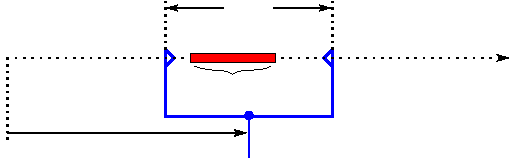
\includegraphics[width=\unitlength]{1dillustration.pdf}}%
    \put(0.15949338,0.01813248){\color[rgb]{0,0,0}\makebox(0,0)[lb]{\smash{$u_2$}}}%
    \put(0.40692504,0.22646518){\color[rgb]{0,0,0}\makebox(0,0)[lb]{\smash{object}}}%
    \put(0.96767264,0.21229788){\color[rgb]{0,0,0}\makebox(0,0)[lb]{\smash{$x$}}}%
    \put(0.44163201,0.13862415){\color[rgb]{0,0,0}\makebox(0,0)[lb]{\smash{$w$}}}%
    \put(0.4455571,0.29089082){\color[rgb]{0,0,0}\makebox(0,0)[lb]{\smash{$u_1$}}}%
    \put(-0.00215418,0.21245965){\color[rgb]{0,0,0}\makebox(0,0)[lb]{\smash{0}}}%
  \end{picture}%
\endgroup%

\captionsetup{justification=raggedright}
\caption{Illustration of a 1-D grasping problem.}
\label{fig:1D_simple}
\end{figure}	

First let us  derive a grasp success probability model $\text{P}(S | x,  \mathcal{G} )$ for this example. Since the positions of the fingertips can determine whether a gripper configuration will succeed, we can compute these positions directly from $u_1$ and $u_2$ by   

%It is obviously that when the  position of the gripper is equal to the position of the object ($u_2 = x$) and the opening width of the gripper is equal to the width of the object ($u_1 = w$), a stable grasp is then established. We define this configuration as a reference $u^{\text{ref}}$: 
%\begin{equation}
%u^{\text{ref}} =  \begin{pmatrix}\begin{figure}
%u_1^{\text{ref}}\\ 
%u_2^{\text{ref}}
%\end{pmatrix}
%=\begin{pmatrix}
%w\\ 
%x
%\end{pmatrix}. 
%\end{equation}
%and assign the probability of grasp success of this configuration with $\text{P}(S | x = x_0, \mathcal{G} = u^{\text{ref}}) = 1$.
\begin{equation}
\begin{pmatrix}
c^{\text{left}}\\ 
c^{\text{right}}
\end{pmatrix}
=\begin{pmatrix}
u_2 - 0.5 \cdot u_1\\ 
u_2 + 0.5 \cdot u_1
\end{pmatrix}.
\end{equation}
If the fingertips are in intersect with the object, the grasp is invalid. In these cases, we assign the probability of grasp success to zero. When the positions of fingertips fulfill the condition ( $c^{\text{left}} < x - 0.5w$ and $c^{\text{right}} > x + 0.5w$ ), the object can be grasped by the gripper. However, for precision grasping, we want to avoid object displacement during grasping. During the phase of force closure, we want the object to move as little as possible. Therefore, a term that penalizes object displacement can be introduced into the grasp success model. We model the grasp success probability by 

\begin{equation}
  \text{P}(S | x,  \mathcal{G} )  = -\frac{1}{ d^{\text{max}} } \cdot d + 1,
  \label{equ:5}
\end{equation}
where $d^{\text{max}}  = 0.5 \cdot (u_{1}^{\text{max}} - w) $ denotes the maximum displacement that can be executed by a gripper. $d = | u_2 - x | $ denotes the actual object displacement. By combining this model with a given object posterior $p(x|\mathcal{Z})$, a marginal success probability $\text{P}(S)$ can be obtained by evaluating Eq.~\ref{e_grasp_success}. To illustrate how an object posterior can influence marginal success probability, we choose object length $w = 0.2$, the maximal opening width of the gripper $u_{1}^{\text{max}} = 0.4 $. We compare the result by using two different object posteriors to simulate an accurate and a less accurate perception system. We model the $p(x|\mathcal{Z})$ by two Gaussian distributions with $\mathcal{N}(0, 0.3)$ and $\mathcal{N}(0, 0.03)$ respectively. Fig.~\ref{fig:1D_grasp} depicts the contour of grasp success probability $\text{P}(S)$ in terms of the pre-touch configuration.

\begin{figure}[!htbp]
\centering
\def\svgwidth{1\linewidth}
%% Creator: Inkscape inkscape 0.48.4, www.inkscape.org
%% PDF/EPS/PS + LaTeX output extension by Johan Engelen, 2010
%% Accompanies image file '1dgrasp_result.pdf' (pdf, eps, ps)
%%
%% To include the image in your LaTeX document, write
%%   \input{<filename>.pdf_tex}
%%  instead of
%%   \includegraphics{<filename>.pdf}
%% To scale the image, write
%%   \def\svgwidth{<desired width>}
%%   \input{<filename>.pdf_tex}
%%  instead of
%%   \includegraphics[width=<desired width>]{<filename>.pdf}
%%
%% Images with a different path to the parent latex file can
%% be accessed with the `import' package (which may need to be
%% installed) using
%%   \usepackage{import}
%% in the preamble, and then including the image with
%%   \import{<path to file>}{<filename>.pdf_tex}
%% Alternatively, one can specify
%%   \graphicspath{{<path to file>/}}
%% 
%% For more information, please see info/svg-inkscape on CTAN:
%%   http://tug.ctan.org/tex-archive/info/svg-inkscape
%%
\begingroup%
  \makeatletter%
  \providecommand\color[2][]{%
    \errmessage{(Inkscape) Color is used for the text in Inkscape, but the package 'color.sty' is not loaded}%
    \renewcommand\color[2][]{}%
  }%
  \providecommand\transparent[1]{%
    \errmessage{(Inkscape) Transparency is used (non-zero) for the text in Inkscape, but the package 'transparent.sty' is not loaded}%
    \renewcommand\transparent[1]{}%
  }%
  \providecommand\rotatebox[2]{#2}%
  \ifx\svgwidth\undefined%
    \setlength{\unitlength}{259.88395945bp}%
    \ifx\svgscale\undefined%
      \relax%
    \else%
      \setlength{\unitlength}{\unitlength * \real{\svgscale}}%
    \fi%
  \else%
    \setlength{\unitlength}{\svgwidth}%
  \fi%
  \global\let\svgwidth\undefined%
  \global\let\svgscale\undefined%
  \makeatother%
  \begin{picture}(1,0.53724423)%
    \put(0,0){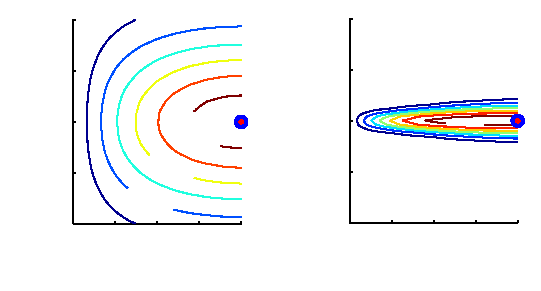
\includegraphics[width=\unitlength]{1dgrasp_result.pdf}}%
    \put(0.1151589,0.08992018){\makebox(0,0)[lb]{\smash{0.2}}}%
    \put(0.18217497,0.08992018){\makebox(0,0)[lb]{\smash{0.25}}}%
    \put(0.27003572,0.08992018){\makebox(0,0)[lb]{\smash{0.3}}}%
    \put(0.33673164,0.08992018){\makebox(0,0)[lb]{\smash{0.35}}}%
    \put(0.4249133,0.08992018){\makebox(0,0)[lb]{\smash{0.4}}}%
    \put(0.08972926,0.1171398){\makebox(0,0)[lb]{\smash{-0.5}}}%
    \put(0.07593948,0.20747584){\color[rgb]{0,0,0}\makebox(0,0)[lb]{\smash{-0.25}}}%
    \put(0.10355064,0.2982193){\makebox(0,0)[lb]{\smash{0}}}%
    \put(0.08669901,0.39782419){\makebox(0,0)[lb]{\smash{0.25}}}%
    \put(0.09666237,0.48644253){\makebox(0,0)[lb]{\smash{0.5}}}%
    \put(0.23790599,0.1699559){\rotatebox{-22.99998994}{\makebox(0,0)[lb]{\smash{0.04}}}}%
    \put(0.27574288,0.23088155){\rotatebox{-25.9999936}{\makebox(0,0)[lb]{\smash{0.08}}}}%
    \put(0.33923275,0.31457275){\rotatebox{-51.0000188}{\makebox(0,0)[lb]{\smash{0.12}}}}%
    \put(0.01695468,0.30375214){\color[rgb]{0,0,0}\makebox(0,0)[lb]{\smash{$u_2$}}}%
    \put(0.27728722,0.04517519){\color[rgb]{0,0,0}\makebox(0,0)[lb]{\smash{$u_1$}}}%
    \put(0.61970258,0.09198088){\makebox(0,0)[lb]{\smash{0.2}}}%
    \put(0.68671864,0.09198088){\makebox(0,0)[lb]{\smash{0.25}}}%
    \put(0.77457939,0.09198088){\makebox(0,0)[lb]{\smash{0.3}}}%
    \put(0.84127531,0.09198088){\makebox(0,0)[lb]{\smash{0.35}}}%
    \put(0.92945698,0.09198088){\makebox(0,0)[lb]{\smash{0.4}}}%
    \put(0.83165564,0.29547016){\rotatebox{-3.00000411}{\makebox(0,0)[lb]{\smash{0.7}}}}%
    \put(0.52418668,0.30637183){\color[rgb]{0,0,0}\makebox(0,0)[lb]{\smash{$u_2$}}}%
    \put(0.7845194,0.05087321){\color[rgb]{0,0,0}\makebox(0,0)[lb]{\smash{$u_1$}}}%
    \put(0.26204153,0.00490434){\color[rgb]{0,0,0}\makebox(0,0)[lb]{\smash{(a)}}}%
    \put(0.79104124,0.0040583){\color[rgb]{0,0,0}\makebox(0,0)[lb]{\smash{(b)}}}%
    \put(0.58730417,0.21390265){\color[rgb]{0,0,0}\makebox(0,0)[lb]{\smash{-0.25}}}%
    \put(0.59889533,0.11916901){\makebox(0,0)[lb]{\smash{-0.5}}}%
    \put(0.61271672,0.30024851){\makebox(0,0)[lb]{\smash{0}}}%
    \put(0.59586509,0.3998534){\makebox(0,0)[lb]{\smash{0.25}}}%
    \put(0.60582844,0.48847175){\makebox(0,0)[lb]{\smash{0.5}}}%
  \end{picture}%
\endgroup%

\caption{ Marginal grasp success probability in terms of two different object posteriors. The optimal gripper configurations are shown by red dots. In (a), $\mathcal{N}(0, 0.3)$ is used to simulate the posterior of the object position. The marginal success probability ${\text{P}(S)}_{u = u_{\text{opt}}} = 0.13$  . In (b) $\mathcal{N}(0, 0.03)$ is used to simulate a more accurate posterior distribution of the object position with ${\text{P}(S)}_{u = u_{\text{opt}}} = 0.76$ }
\label{fig:1D_grasp}
\end{figure}	 


\subsection{Modelling of conditional grasp success probability } \label{sec:grasp_success_model}
For real world objects, it is required to have a conditional grasp success model that consider much more factors than the 1-D example, so that the conditional grasp success model can approximate the true probability. Two conditions are necessary to ensure a successful grasp. First, the motion of a gripper, which is represented by $\mathcal{G}$, should not collide with the environment and the object. Second, the last pose and posture $g_n$ which we define as the pre-touch configuration should guarantee that forces from the fingertips are established on the object in the third phase. For the first condition, we assume that there is sufficient free space between the pre-grasp configuration and the pre-touch configuration. The collision-free motion from the pre-grasp to the pre-touch can be computed using a pre-defined heuristic: approaching with a linear motion. To fulfill the second condition, the choice of a pre-touch configuration $g_n$ is essential, because the grasp success is predominantly affected by the way we make contact with the object. Hence, the grasp success model $P(S | x,\mathcal{G})$ is simplified to $P(S | x, g_n$). 

The dimension of the object state $x$ depends on the choice of an object representation. To represent simple geometry primitives such as cylindrical objects, it is sufficient to choose a parametric representation which includes radius, height, and the position of the object. For objects which form are irregular, the dimension of $x$ can be very large. However, predicting the grasp success probability can be independent of the choice of representation, since it is only required to extract the contact normals of an object.  

In the following, we elaborate on how we calculate the conditional success probability of a pre-touch configuration $g_n$ for real world objects. Here we only study the pinch grasp, that a grasp only requires two fingers to make contact with the object. Pinch grasp can be easily realized by most grippers, independent of how many fingers a gripper having. We choose four criteria to model the conditional grasp success probability. 

\begin{figure}[!htbp]
\centering
\def\svgwidth{0.7\linewidth}
%% Creator: Inkscape inkscape 0.48.4, www.inkscape.org
%% PDF/EPS/PS + LaTeX output extension by Johan Engelen, 2010
%% Accompanies image file 'bunny.pdf' (pdf, eps, ps)
%%
%% To include the image in your LaTeX document, write
%%   \input{<filename>.pdf_tex}
%%  instead of
%%   \includegraphics{<filename>.pdf}
%% To scale the image, write
%%   \def\svgwidth{<desired width>}
%%   \input{<filename>.pdf_tex}
%%  instead of
%%   \includegraphics[width=<desired width>]{<filename>.pdf}
%%
%% Images with a different path to the parent latex file can
%% be accessed with the `import' package (which may need to be
%% installed) using
%%   \usepackage{import}
%% in the preamble, and then including the image with
%%   \import{<path to file>}{<filename>.pdf_tex}
%% Alternatively, one can specify
%%   \graphicspath{{<path to file>/}}
%% 
%% For more information, please see info/svg-inkscape on CTAN:
%%   http://tug.ctan.org/tex-archive/info/svg-inkscape
%%
\begingroup%
  \makeatletter%
  \providecommand\color[2][]{%
    \errmessage{(Inkscape) Color is used for the text in Inkscape, but the package 'color.sty' is not loaded}%
    \renewcommand\color[2][]{}%
  }%
  \providecommand\transparent[1]{%
    \errmessage{(Inkscape) Transparency is used (non-zero) for the text in Inkscape, but the package 'transparent.sty' is not loaded}%
    \renewcommand\transparent[1]{}%
  }%
  \providecommand\rotatebox[2]{#2}%
  \ifx\svgwidth\undefined%
    \setlength{\unitlength}{194bp}%
    \ifx\svgscale\undefined%
      \relax%
    \else%
      \setlength{\unitlength}{\unitlength * \real{\svgscale}}%
    \fi%
  \else%
    \setlength{\unitlength}{\svgwidth}%
  \fi%
  \global\let\svgwidth\undefined%
  \global\let\svgscale\undefined%
  \makeatother%
  \begin{picture}(1,0.67409794)%
    \put(0,0){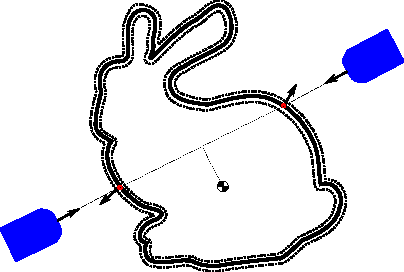
\includegraphics[width=\unitlength]{bunny.pdf}}%
    \put(0.12693299,0.16410315){\color[rgb]{0,0,0}\makebox(0,0)[lb]{\smash{$n_1$}}}%
    \put(0.7863913,0.49764194){\color[rgb]{0,0,0}\makebox(0,0)[lb]{\smash{$n_2$}}}%
    \put(0.64071158,0.3573397){\color[rgb]{0,0,0}\makebox(0,0)[lb]{\smash{$c_2$}}}%
    \put(0.31678681,0.21094795){\color[rgb]{0,0,0}\makebox(0,0)[lb]{\smash{$c_1$}}}%
    \put(0.19497423,0.18987635){\color[rgb]{0,0,0}\makebox(0,0)[lb]{\smash{$d_1$}}}%
    \put(0.76565879,0.40945617){\color[rgb]{0,0,0}\makebox(0,0)[lb]{\smash{$d_2$}}}%
  \end{picture}%
\endgroup%

\caption{Description of variables which represent a pre-touch configuration $g_n$ on an bunny object. Fingertips are illustrated in blue. Dashed lines indicate variances of the representation. Arrows represent normals on the particular surfaces.}
\label{fig:grasp_generation}
\end{figure}

\begin{itemize}
\item \textit{Non-zero contact angle}: 
 The first criterion that affects the grasp success is the angle between normal of fingertips and desired contact regions. In Fig.~\ref{fig:grasp_generation}, we denote $n_i$ as the normal defined on a finger tip and $c_i$ as the normal of a contact region. $d_i$ is the distance from a finger tip to a contact region. The grasp success probability with a non-zero contact angle is given by:
\begin{equation}
P_1 = \begin{cases}
\prod_{i=1}^{k}(1 -\frac{1}{0.5\cdot \theta} |\beta|)   & |\beta | < \frac{\theta}{2}\\
  0   & \text{else}
\end{cases},
\end{equation} 
where $\beta = \pi - \angle(n_i,c_i)$ and $\angle(n_i,c_i)$ is the angle between $n_i$ and $c_i$.  $k$ denotes the total number of fingertips used to make contact with the object. $\theta$ is the maximal angle of a friction cone that the finger tip still supports the object without slipping. 
\item \textit{Non-optimal finger placement}:
Due to the non-optimal control of a gripper during force closure, the closer the fingertips are located to the object surface, the less likely a control error would occur to influence the overall grasp success. Therefore this criterion is modeled by 
\begin{equation} 
P_2 = \text{exp}\left(-\sum_{i=1}^k \frac{d_i-h}{\sigma_h^2}\right)
\end{equation}
where $h$ is the desired offset distance between fingertips and the object's surface for a pre-touch configuration. $\sigma_h$ is a shaping factor for the probability. 

\item \textit{Distance to center of gravity}:
This criterion penalizes a grasp that the line connecting two contact points does not cross an object's center of gravity. A large distance between the center of gravity to the line may result in that the object rotates within the gripper after being lifted up.  We model success probability of this criterion by 
\begin{equation} 
P_3 = \begin{cases}
  1 -\frac{1}{ 0.5\cdot l_{bb} } |d_{\text{cg}}|      &  |d_{\text{cg}}|   < 0.5 \cdot l_{bb}  \\
  0   & \text{else}
\end{cases},
\end{equation}
where $d_{\text{cg}}$ denotes the distance from the line of contact points to an object's center of gravity. For unknown objects, we do not know  exactly where the center of gravity lies. However, based on the reconstructed object model we can fit a bounding box to the object. The center  of the bounding box is a good estimate of the center of gravity.  $l_{bb}$ is the largest side length of the bounding box. We use a heuristic to penalize the distance larger than the half of the side length. 

\item \textit{Surface uncertainty}:
 This criterion is specially designed for the representation that models surface uncertainty. This criterion avoids making the finger contact on uncertain surfaces because forces established on uncertain surfaces can not guarantee firm touch between the fingertips and the object. We model the success probability induced by surface uncertainty with 
\begin{equation}
 P_4 =  \begin{cases}
\prod_{i=1}^{k}(1 -\frac{\mean{\sigma(c_i)}}{\sigma_{\text{max}} }   )  &  \mean{\sigma(c_i)} < \sigma_{\text{max}}\\
  0   & \text{else}
\end{cases},
\end{equation} 
where $\mean{\sigma(c_i)} $ is an average variance of $c_i$ and $\sigma_{\text{max}}$ is a parameter representing the maximal allowed variance. We merge the proposed  criteria in a weighted fashion to generate an overall grasp success probability by  
\begin{equation}
P(S | x , g_n) =  \sum_{i=1}^4 w_i \cdot P_i 
\label{equ:weights}
\end{equation} 
with $\sum_{i=1}^4 w_i  = 1$.
\end{itemize}


\section{Modelling perception uncertainty}

%\subsection{Shape-primitive based probability distribution estimation using extended Kalman filter}


\subsection{Surface based probability distribution estimation based on probabilistic fusion}
The aforementioned shape-based approach that aims to represent the object with a limited number of parameters does not scale to real world objects. The reason is that the shapes and surfaces of most real world objects are complex and individual. Grasping these objects requires a robot to have the capability of learning the form of irregular objects online even the object is presented for the first time. In this section, we propose a new method to estimate the probability distribution of the surface of the objects. Rather than predict the shape parameter, this method estimates the course of the object surface achieved by a new probabilistic object representation and a multi-sensor fusion approach. Our surface representation has some significant advantages. First, it models the measurement uncertainty explicitly, as the fusion method explicitly takes Second, the model can be reconstructed with multiple measurements generated by various sensors, which have different noise characteristics. Third, one can parallelize the fusion method on GPU, so that the reconstruction
process is performed in real time. Fourth, the efficient query of the surface information allows fast grasp synthesis.

\subsection{Surface representation: p-SDF}
The model of the surface representation is based on signed distance field (SDF). A SDF in a metric space determines the distance between a point and the object surface. The sign of the distance indicates whether the point is outside or inside the object. Besides the distance information, we augment the SDF with another additional variable $\sigma$ to represent the uncertainty of the distance. We call this new probabilistic surface representation p-SDF. In this work, a discretized version of p-SDF is used. We discretize a predefined metric space, where p-SDF is defined, into equally sized voxels. We denote the set of all the voxels as $V$. Since the modeling of an object can never be perfect, we have to take the surface uncertainty of modeling into account. For this purpose, we define the distance to each voxel as a normal-distributed random variable. Thus, an object is represented by  
\begin{equation}
\bm{f}: v \mapsto \mathcal{N}(\mu, \sigma^2),  \forall v \in  V ,
\end{equation}
where $\mu$ is the mean and $\sigma$ is the variance of the distribution assigned to voxel $v$.  

\subsection{Surface reconstruction with sensor fusion}
In order to fuse the measurements into the representation using multiple sensors, an iterative method is used to update all the voxel elements. Considering only one voxel $v\in V$, we introduce a  random variables $D_{k}$ associated with voxel $v$. Here, $k$ denotes a time stamp. $\text{Bel}(D_{k-1})$ and $\text{Bel}(D_{k})$ represent the belief signed distance distributions at time stamp $k-1$ and $k$ respectively. We also assume that the major error of one sensor measurement can be approximated as Gaussian white noise so that we can define a measurement model of the sensor by 
\begin{equation}
\text{P}(z|c,\Omega) = \mathcal{N}(z^*,  \sigma_\text{sensor}^2), 
\end{equation}
where $c$ denotes a depth camera pose and $\Omega$ denotes the surface of an object. $z^*$ is the true distance between the surface and the depth camera. Furthermore, we denote the true distance between the voxel $v$ to the surface $\Omega$ as $z_\text{sdf}^*$. From Fig.~\ref{fig:sdf} we can derive 
\begin{equation}
z_\text{sdf}^*  = d_{( v,c) } - z^*
\end{equation}
where $d_{( v,c) }$ denotes the distance between the voxel $v$ and the depth camera. Since $z$ follows a Gaussian distribution, $z_\text{sdf}$ also follows a Gaussian distribution, which is given by 
\begin{equation}
\text{P}(z_\text{sdf}|c,\Omega) = \mathcal{N}(z_\text{sdf}^*,  \sigma_\text{sensor}^2).
\end{equation}

\begin{figure}[!htbp]
\centering
\def\svgwidth{0.8\linewidth}
%% Creator: Inkscape inkscape 0.48.3.1, www.inkscape.org
%% PDF/EPS/PS + LaTeX output extension by Johan Engelen, 2010
%% Accompanies image file 'sdf.pdf' (pdf, eps, ps)
%%
%% To include the image in your LaTeX document, write
%%   \input{<filename>.pdf_tex}
%%  instead of
%%   \includegraphics{<filename>.pdf}
%% To scale the image, write
%%   \def\svgwidth{<desired width>}
%%   \input{<filename>.pdf_tex}
%%  instead of
%%   \includegraphics[width=<desired width>]{<filename>.pdf}
%%
%% Images with a different path to the parent latex file can
%% be accessed with the `import' package (which may need to be
%% installed) using
%%   \usepackage{import}
%% in the preamble, and then including the image with
%%   \import{<path to file>}{<filename>.pdf_tex}
%% Alternatively, one can specify
%%   \graphicspath{{<path to file>/}}
%% 
%% For more information, please see info/svg-inkscape on CTAN:
%%   http://tug.ctan.org/tex-archive/info/svg-inkscape
%%
\begingroup%
  \makeatletter%
  \providecommand\color[2][]{%
    \errmessage{(Inkscape) Color is used for the text in Inkscape, but the package 'color.sty' is not loaded}%
    \renewcommand\color[2][]{}%
  }%
  \providecommand\transparent[1]{%
    \errmessage{(Inkscape) Transparency is used (non-zero) for the text in Inkscape, but the package 'transparent.sty' is not loaded}%
    \renewcommand\transparent[1]{}%
  }%
  \providecommand\rotatebox[2]{#2}%
  \ifx\svgwidth\undefined%
    \setlength{\unitlength}{237.96421848bp}%
    \ifx\svgscale\undefined%
      \relax%
    \else%
      \setlength{\unitlength}{\unitlength * \real{\svgscale}}%
    \fi%
  \else%
    \setlength{\unitlength}{\svgwidth}%
  \fi%
  \global\let\svgwidth\undefined%
  \global\let\svgscale\undefined%
  \makeatother%
  \begin{picture}(1,0.57494457)%
    \put(0,0){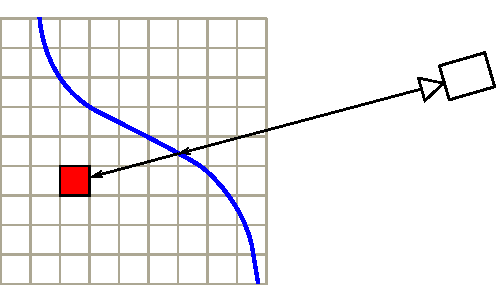
\includegraphics[width=\unitlength]{sdf.pdf}}%
    \put(0.18274527,0.37685155){\color[rgb]{0,0,0}\makebox(0,0)[lb]{\smash{$\Omega$}}}%
    \put(0.59084169,0.36325775){\color[rgb]{0,0,0}\makebox(0,0)[lb]{\smash{$z^*$}}}%
    \put(0.23977624,0.19236224){\color[rgb]{0,0,0}\makebox(0,0)[lb]{\smash{$z_\text{sdf}^*$}}}%
    \put(0.14259879,0.20147031){\color[rgb]{0,0,0}\makebox(0,0)[lb]{\smash{$v$}}}%
    \put(0.89596954,0.33036162){\color[rgb]{0,0,0}\makebox(0,0)[lb]{\smash{$c$}}}%
    \put(0.00452449,0.54940239){\color[rgb]{0,0,0}\makebox(0,0)[lb]{\smash{$V$}}}%
  \end{picture}%
\endgroup%

\caption{Description of the variables that we defined. The grid denotes the volume we consider for modelling an object. $z^*$ is the true measurement from a depth camera. $c$ denotes the pose of the depth camera. $ z_\text{sdf}^*$ is the true signed distance along the direction of the measurement.}
\label{fig:sdf}
\end{figure}	

The belief distribution  $\text{Bel}(D_{k})$ of voxel $v$ can be derived by Bayesian recursive updating by   


\begin{equation}
\begin{split}
\text{Bel}(D_{k}) &= \text{P}(D_{k} | z_\text{sdf}^1,\cdots, z_\text{sdf}^k) \\
                  &= \eta \cdot \text{P}(z_\text{sdf}^k | D_{k} ) \cdot  \text{P}(D_{k-1}|z_\text{sdf}^1\cdots z_\text{sdf}^{k-1} )  \\
                  &= \eta \cdot \text{P}(z_\text{sdf}^k | D_{k} ) \cdot \text{Bel}(D_{k-1})
  \end{split}
\end{equation}   
This equation shows that $\text{Bel}(D_{k})$ can be computed iteratively by the measurement model and the belief prior to the measurement update. In this work, we propose to approximate the belief with a Gaussian distribution for each voxel, so the belief  $\text{Bel}(D_{k})$ can be further computed by 

\begin{equation}
\begin{split}
\text{Bel}(D_{k}) &= \eta \cdot \mathcal{N}(z_\text{sdf},  \sigma_\text{sensor}^2) \cdot  \mathcal{N}( \mu_{k-1} ,   \sigma_{k-1} ^2) \\
&= \eta' \cdot \mathcal{N}( \mu_{k} ,   \sigma_{k} ^2)
  \end{split}
\end{equation}   

with 

\begin{equation}
\label{equ:rule1}
\begin{split}
  {\mu}_{k} &= \frac{{\mu}_{k-1}\cdot\sigma_\text{sensor}^{2}+  z_\text{sdf} \cdot\sigma_{k-1}^{2}}{\sigma_{k-1}^{2}+\sigma_\text{sensor}^2}
\end{split}
\end{equation}
%
\begin{equation}
\label{equ:rule2}
\begin{split}
  \sigma_{k}^{2} &=\frac{\sigma_{k-1}^{2}\cdot\sigma_\text{sensor}^2}{\sigma_{k-1}^{2}+\sigma_\text{sensor}^2}.
\end{split}
\end{equation}
We use Equ.~\ref{equ:rule1} and Equ.~\ref{equ:rule2} to update the whole volume $V$. To update the volume with another depth camera, one only needs to exchange $\sigma_\text{sensor}^2$ to the variance which represents the measurement characteristics of the camera. 



\section{Searching for feasible grasp configuration}

In general, numerous pre-touch configurations are feasible for a successful grasp, since most objects can be stably grasped in different ways. The marginal probability $P(s|g_n,\bm{f})$ is a high-dimensional non-convex function on $g_n$. $g_n$ is parameterized by the pose of the gripper relatively to the object and the positions of joints. Finding the optimum of $g_n$ is not trivial. We propose to solve this problem in two steps. First, we use a generalizable method to parameterize the grasping posture which reduces the dimension of gripper configurations. The parametrization is then used in a two-stage search process, which involves sampling many configurations to evaluate the success probability and refining the configuration of the best sample.    

\subsection{Reducing configuration space of grippers using synergy }\label{sec:gripper_parametrization}

We follow the concept of `eigen-grasp'\cite{Ciocarlie2009} to parameterize the gripper. This concept is based on the grasp synergy which allows the joint positions to be controlled only by a subspace of the total available degrees of freedom. In our work, we use grippers with more than two degrees of freedom (DOF). Given a gripper with $d$ DOF, we organize joints on the same finger into a group so that only one parameter is required to control the whole finger. We define the set of joint groups as $\mathbb{J}$. Later we use this reduced parameter space to search for grasps. After defining the groups, we define a set of grasp types $\mathbb{T}$ that are feasible for the gripper. Typically, they indicate which grasp type is reasonable for a specific object or a specific task, e.g. a pinch grasp is more suitable for grasping a chopstick than a power grasp. A grasp type is parametrized by an opening posture $P_b \in\mathbb{R}^d$  and a closing posture $P_e \in\mathbb{R}^d$. To generate a gripper configuration of a particular type, we must first compute an eigen grasp matrix  $M$ for this type. The algorithm for computing $M$ is given by Algorithm \ref{alg1}. 

\begin{algorithm}
\begin{algorithmic}[1]
\STATE Input:  $\mathbb{J}$, $P_b$, $P_e$, $d$   
\STATE $n_g  =  |\mathbb{J}| $
\STATE $k = 0$ % joint index
\STATE $r = 0$ % row begin 
\STATE resize $M$ to $d$ rows and $n_g$ columns  
\FOR {$i$ from 1 to $n_g$}
\FOR {$j$ from 1 to $\mathbb{J}$[i] }
\STATE row = $r + j$ 
\STATE col = $i$   
\STATE $M$(row, col) = $P_e[k] - P_b[k]$
\STATE $k = k + 1$
\ENDFOR
\STATE $r = r + n_g$
\ENDFOR
\RETURN $M$
%\captionsetup{justification=raggedright}
\caption {Compute $M_t$ of grasp type $t$}
\label{alg1}
\end{algorithmic}
\end{algorithm}

The entire joint configuration of a grasp $\bm{j}$ is computed by 
\begin{equation}
\bm{j} = M \cdot \alpha + P_b
\label{equ:eigen_grasp}
\end{equation}
where $M$ is a $d \times n_g$ matrix, $\alpha$ is a $n_g \times 1$ vector and $n_g$ is the number of groups we defined for the gripper. Also note that $\forall \alpha_i \in \alpha, \alpha_i$ is defined in $[0,1]$. Thus the joint configuration $j$ equals $P_b$ when $\forall \alpha_i \in \alpha$, $\alpha_i = 0$ and equals $P_e$ when $\forall \alpha_i \in \alpha$, $\alpha_i = 1$. 

\begin{figure}[!htbp]
\centering
\def\svgwidth{1\linewidth}
%% Creator: Inkscape inkscape 0.48.3.1, www.inkscape.org
%% PDF/EPS/PS + LaTeX output extension by Johan Engelen, 2010
%% Accompanies image file 'grasp_types_new.pdf' (pdf, eps, ps)
%%
%% To include the image in your LaTeX document, write
%%   \input{<filename>.pdf_tex}
%%  instead of
%%   \includegraphics{<filename>.pdf}
%% To scale the image, write
%%   \def\svgwidth{<desired width>}
%%   \input{<filename>.pdf_tex}
%%  instead of
%%   \includegraphics[width=<desired width>]{<filename>.pdf}
%%
%% Images with a different path to the parent latex file can
%% be accessed with the `import' package (which may need to be
%% installed) using
%%   \usepackage{import}
%% in the preamble, and then including the image with
%%   \import{<path to file>}{<filename>.pdf_tex}
%% Alternatively, one can specify
%%   \graphicspath{{<path to file>/}}
%% 
%% For more information, please see info/svg-inkscape on CTAN:
%%   http://tug.ctan.org/tex-archive/info/svg-inkscape
%%
\begingroup%
  \makeatletter%
  \providecommand\color[2][]{%
    \errmessage{(Inkscape) Color is used for the text in Inkscape, but the package 'color.sty' is not loaded}%
    \renewcommand\color[2][]{}%
  }%
  \providecommand\transparent[1]{%
    \errmessage{(Inkscape) Transparency is used (non-zero) for the text in Inkscape, but the package 'transparent.sty' is not loaded}%
    \renewcommand\transparent[1]{}%
  }%
  \providecommand\rotatebox[2]{#2}%
  \ifx\svgwidth\undefined%
    \setlength{\unitlength}{221.55bp}%
    \ifx\svgscale\undefined%
      \relax%
    \else%
      \setlength{\unitlength}{\unitlength * \real{\svgscale}}%
    \fi%
  \else%
    \setlength{\unitlength}{\svgwidth}%
  \fi%
  \global\let\svgwidth\undefined%
  \global\let\svgscale\undefined%
  \makeatother%
  \begin{picture}(1,0.57628075)%
    \put(0,0){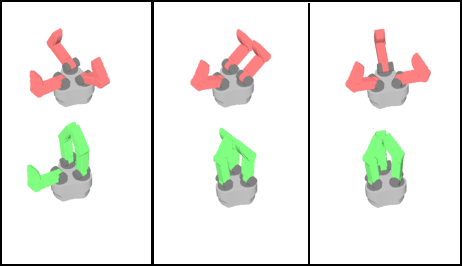
\includegraphics[width=\unitlength]{grasp_types_new.pdf}}%
    \put(0.09508525,0.04601723){\color[rgb]{0,0,0}\makebox(0,0)[lb]{\smash{pinch}}}%
    \put(0.45764631,0.04601723){\color[rgb]{0,0,0}\makebox(0,0)[lb]{\smash{cylindrical}}}%
    \put(0.8037149,0.04601723){\color[rgb]{0,0,0}\makebox(0,0)[lb]{\smash{spherical}}}%
  \end{picture}%
\endgroup%

%\captionsetup{justification=centering}
\caption{Three grasp types are defined for SCHUNK-SDH gripper. The fingers of the gripper for an opening grasp posture $P_b$ are marked in red, the ones for a closing grasp posture $P_e$ are marked in green.}
\label{fig:grasp_types}
\end{figure}	

Fig.~\ref{fig:grasp_types} depicts an example how we parametrize a SCHUNK-SDH gripper. SCHUNK-SDH has a total of three fingers. Each of them has two joints with independent actuators. Two of three fingers have an additional joint at the finger root. These two joints are driven by the same actuator to change the directions of force closure. We define in total three grasp types and their corresponding parameters $P_b$ and $P_e$. We organize two joints on the same finger into one group and additionally the two coupled joints into another group. The total amount of the joint groups adds up to four for this gripper. In this work, we focus on the pinch grasp only, since it mimics the most widely used parallel gripper and is capable of picking a large amount types of objects.  

\subsection{Calculation of surface normals}
Surface normals on the desired contact points are used to evaluate the conditional grasp success probability. For the objects which can be represented by p-SDF, the surface element can be accessed by an operation called ray-casting. Ray casting evaluates the function along a given direction until a zero-crossing is found. To employ this method for grasp generation, we attach a set of frames organized by a grid to each finger tip. These frames are then used as a set of simulated proximity sensors to determine the distance between fingertips and the object surface. The region covered by these frames can be considered as a desired contact patch region. Fig. \ref{fig:simulated_sensor} depicts a realization of simulated proximity sensors on a SCHUNK-SDF Gripper.

\begin{figure}[!htbp]
\centering
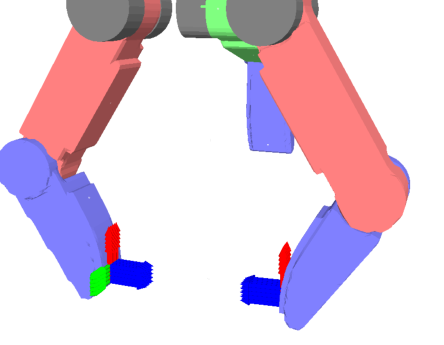
\includegraphics[width=0.4\linewidth]{camera_frame2.pdf}
\captionsetup{justification=raggedright}
\caption{For each finger tip, 25 Frames are attached to the region, where contacts and forces are applied during grasping.}
\label{fig:simulated_sensor}       % Give a unique label
\end{figure}   

Given an object modeled by p-SDF and a pre-touch configuration of a gripper, the desired contact normals are evaluated by first conducting ray casting for each frame. We obtain 25 desired contact points which form a contact region.  We use these points as inputs for a RANSAC plane segmentation \cite{Zuliani2008}. The contact region is regarded as feasible, if at least 20 points are considered as inlier of a plane. This rules out unstable contact region where the course of an object surface is not smooth. The normal of the contact can be calculated from the plane segmentation result. In this way, we avoid using a point-contact model to evaluate contacts but use a contact patch for estimating the contacts and contact normals. It simulates physical contacts in a real grasping scenario. Stable contacts are usually established on the plane of two surfaces, not on the point.  Fig.~\ref{fig:bunny_raycast} depicts the result of the contact points (magenta) and surface normals (yellow arrows) determined by ray casting.

\begin{figure}[!htbp]
\centering
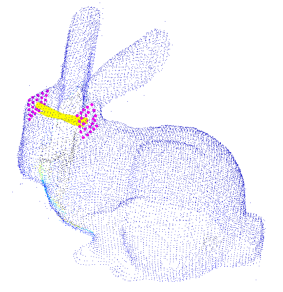
\includegraphics[width=0.4\linewidth]{bunny_raycast_new.pdf}
\captionsetup{justification=raggedright}
\caption{Desired contact positions of a pre-touch configuration determined by ray casting. Magenta: contact points, yellow arrows: surface normals. For  the purpose of visualization, this model is generated in Gazebo simulation.}
\label{fig:bunny_raycast}       % Give a unique label
\end{figure} 


\subsection{A two-stage method for grasp synthesis}
The objective function $P(S | g_n, \bm{f})$ to be maximized is in general non-linear and non-convex. Directly searching in the parameter space tends to find local-optimal solutions. The parameter space of $g_n = \lbrace \bm{p}, \bm{\alpha} \rbrace $ contains a pose parameter $\bm{p}$ in $\mathbb{R}^6$ and a posture parameter $\bm{\alpha}$ in $\mathbb{R}^{N_g}$. The pose parameter can be used to place the gripper at an almost satisfactory region, in which simulated proximity sensors have valid measurements,  while the posture parameter is used for the fine adjustment of the fingertips. In algorithm 2, we propose a two-stage method to generate the pre-touch configuration. In the first stage, we sample a set of new poses based on an input parameter $\Delta d$ from a uniform distribution. $\Delta d$ can be chosen as the largest length of the bounding box of the object, which we obtained from a segmented point cloud. Then we apply the offsets sampled from the distribution to the initial configuration $g_{\text{init}}$ to generate a set of sample configurations. All the samples are then evaluated in Line 9 and 10. The function IK$(g_{\text{sample}})$ checks if the sample configuration is reachable of the robot and collision-free from the environment. The sample with the largest marginal success probability is then passed to stage 2 of the algorithm. In stage 2, we refine the pre-touch configuration from the result of stage 1.  We sample the poses within the XZ plane of the gripper by parameter $\Delta d_r$. We choose parameter $\Delta d_r$ to be sufficiently small (e.g 1 cm) but still give the algorithm the opportunity to find a better pre-touch configuration. The intuition behind that is a better pre-touch configuration can be found within a neighbored region of the pose of $g^*$ from stage 1. From Line 25 to Line 29, we evaluate the distance from the fingertips to the surface and use this information to iteratively search for the posture parameter $\bm{\alpha}$ until the distance is within the threshold of a desired pre-touch configuration distance $d_{\text{pre}}$.

\begin{figure}[!htbp]
\centering
\def\svgwidth{0.4\linewidth}
%% Creator: Inkscape inkscape 0.48.4, www.inkscape.org
%% PDF/EPS/PS + LaTeX output extension by Johan Engelen, 2010
%% Accompanies image file 'algorith_help.pdf' (pdf, eps, ps)
%%
%% To include the image in your LaTeX document, write
%%   \input{<filename>.pdf_tex}
%%  instead of
%%   \includegraphics{<filename>.pdf}
%% To scale the image, write
%%   \def\svgwidth{<desired width>}
%%   \input{<filename>.pdf_tex}
%%  instead of
%%   \includegraphics[width=<desired width>]{<filename>.pdf}
%%
%% Images with a different path to the parent latex file can
%% be accessed with the `import' package (which may need to be
%% installed) using
%%   \usepackage{import}
%% in the preamble, and then including the image with
%%   \import{<path to file>}{<filename>.pdf_tex}
%% Alternatively, one can specify
%%   \graphicspath{{<path to file>/}}
%% 
%% For more information, please see info/svg-inkscape on CTAN:
%%   http://tug.ctan.org/tex-archive/info/svg-inkscape
%%
\begingroup%
  \makeatletter%
  \providecommand\color[2][]{%
    \errmessage{(Inkscape) Color is used for the text in Inkscape, but the package 'color.sty' is not loaded}%
    \renewcommand\color[2][]{}%
  }%
  \providecommand\transparent[1]{%
    \errmessage{(Inkscape) Transparency is used (non-zero) for the text in Inkscape, but the package 'transparent.sty' is not loaded}%
    \renewcommand\transparent[1]{}%
  }%
  \providecommand\rotatebox[2]{#2}%
  \ifx\svgwidth\undefined%
    \setlength{\unitlength}{101.7223632bp}%
    \ifx\svgscale\undefined%
      \relax%
    \else%
      \setlength{\unitlength}{\unitlength * \real{\svgscale}}%
    \fi%
  \else%
    \setlength{\unitlength}{\svgwidth}%
  \fi%
  \global\let\svgwidth\undefined%
  \global\let\svgscale\undefined%
  \makeatother%
  \begin{picture}(1,1.11202323)%
    \put(0,0){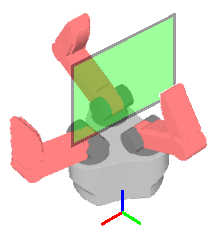
\includegraphics[width=\unitlength]{algorith_help.pdf}}%
    \put(0.61706548,0.89542968){\color[rgb]{0,0,0}\makebox(0,0)[lb]{\smash{xz plane}}}%
    \put(0.43200533,0.02430309){\color[rgb]{0,0,0}\makebox(0,0)[lb]{\smash{x}}}%
    \put(0.66835092,0.01635887){\color[rgb]{0,0,0}\makebox(0,0)[lb]{\smash{y}}}%
    \put(0.5572892,0.21926022){\color[rgb]{0,0,0}\makebox(0,0)[lb]{\smash{z}}}%
  \end{picture}%
\endgroup%

%\captionsetup{justification=centering}
\caption{Parametrization for refining a pre-touch configuration.}
\label{fig:algorith_help}
\end{figure}	



\begin{algorithm}
\begin{algorithmic}[1]
\STATE Input: $\bm{f} $, $g_{\text{init}}$,  $N_{\text{sample}}$ , $N_{\text{refine}}$, $\Delta d$ , $\Delta d_r$, $d_{\text{pre}}$
\STATE $P^{*} = 0$
\STATE $\Delta \bm{\alpha} = [0.01, 0.01]$
\STATE // stage 1.
\FOR { $i$ from 1 to $N_{\text{sample}}$ } 
\STATE   Sample offsets $\Delta x^{*}$,$\Delta y^{*}$,$\Delta z^{*}$ from  Unif(-$\frac{\Delta d}{4} ,+ \frac{\Delta d}{4}$)
\STATE   Sample $\Delta \beta$ from Unif(-$\pi ,+ \pi$)
\STATE   $g_{\text{sample}} \leftarrow $ Apply position offsets and  rotation offset $\Delta \beta$ to $g_{\text{init}}$ 
\STATE  $P_i = P(S | g_{\text{sample}}, \bm{f})$
\IF {  $P_i > P^{*} $ and IK  ($g_{\text{sample}}$ ) is True}
\STATE $P^{*} = P_i$
\STATE $g^{*} = g_{\text{sample}} $
\ENDIF  
\ENDFOR 
\STATE // stage 2
\FOR { $j$ from 1 to $N_{\text{refine}}$ } 
\STATE Sample an offset from Unif( -$\Delta d_r$ ,$\Delta d_r$ )
\STATE $g_{\text{refine}} \leftarrow $ Apply the offset to pose of $g^{*}$ in xz plane (see. Fig.~\ref{fig:algorith_help})  
\STATE  $P_{\text{refine}} = P(S | g_{\text{refine}}, \bm{f})$
\IF {  $P_{\text{refine}} > P^{*} $ }
\STATE $P^{*} = P_{\text{refine}}$
\STATE $g^{*} = g_{\text{refine}} $
\ENDIF
\ENDFOR
\STATE $(d_1,d_2) = \text{raycast}(g^*, \bm{f})$
\WHILE { $ |d_1 - d_{\text{pre}}| > 1 mm$ or $ |d_2 - d_{\text{pre}}| >1 mm$ }
\STATE $y_{(g^{*})} = y_{(g^{*})} + \frac{d_1-d_2}{2} $ 
\STATE $ \bm{\alpha}_{(g^*)} = \bm{\alpha}_{(g^*)} + \Delta \bm{\alpha}$ 
\STATE $(d_1,d_2) = \text{raycast}(g^*, \bm{f})$
\ENDWHILE
\RETURN $g*$
\caption {A two-stage pre-touch generation algorithm for pinch grasp}
\end{algorithmic}
\end{algorithm}

\section{Experimental evaluation: Grasping unknown objects}
We choose a challenging task, grasping of unknown objects, to validate the proposed approach. Unknown objects are the objects which are presented to a robot for the first time. All of the objects we chose for this experiment have their individual shapes, which additionally increase the difficulty. In the following, we first introduce the experimental setup, followed by the evaluation of the algorithm and the performance evaluation of the overall grasping accuracy. 

\subsection{Experimental setup}
The test objects that we used in the experiment are shown in Fig.~\ref{fig:test_objects}. Every time we place one object on the table. The robot is required to lift the object 10 cm above the table. If the robot grasps the object successfully, it rotates its wrist of a random angle and places the object back to start a new grasping attempt. For each object, the robot repeats the experiment autonomously for 20 attempts. Human intervention is only involved if the robot fails to pick up an object. In the case that the robot does not recognize the failure and continues to place back the object,  we manually remove the object to prevent the robot from breaking its gripper.  

\begin{figure}[!htbp] 
\centering
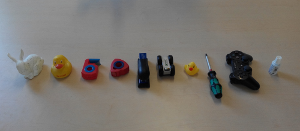
\includegraphics[width=0.7\linewidth]
{figure/test_object.png}%\captionsetup{justification=centering}
\caption{Test objects we used in this experiment. From left to right: a 3-D printed `bunny', `big duck', `tape rectangular', `tape triangle', `stapler', `toy car', `duckie', `screwdrawer', `PS3 joystick', `correction fluid'. }
\label{fig:test_objects}
\end{figure}	
   
\subsubsection{Hardware}
We conduct the experiments with a fully integrated mobile manipulation robot (Care-o-bot)~\cite{careobot}. The robot is equipped with a 7 DOF KUKA lightweight robot with a 7 DOF SCHUNK-SDH gripper mounted on the wrist. The robot is driven by an omnidirectional mobile platform. The primary sensors of the robot include a head-mounted Microsoft Kinect sensor and a hand-mounted stereo camera (Ensenso N10). 

\subsubsection{Object modelling}
Before each grasp attempt, the robot moves its gripper to several pre-defined poses so that the object is perceived from both head camera (Kinect) and in-hand camera (Ensenso). During the movement, our fusion algorithm integrates the measurements simultaneously from both cameras. Fig.~\ref{fig:time_evolution} illustrates the process of modeling the `toy car' by moving the gripper relatively slowly. For the first 9 s, the top side of the object is visible to the in-hand camera, so the uncertainty of the top region is reduced gradually. The black area of the object indicates that the region of wheels is still under large uncertainty. After 9 s the robot moves the in-hand camera to some other viewpoints to acquire more information about the region of wheels. Fig.~\ref{fig:numberofframes} shows the number of frames used to fuse the object during the entire modeling process.  

\begin{figure}[!htbp]
\centering
%\def\svgwidth{1\linewidth}
\includegraphics[width=1\linewidth]{figure/time_evolution.png}%\captionsetup{justification=centering}
%%% Creator: Inkscape inkscape 0.48.4, www.inkscape.org
%% PDF/EPS/PS + LaTeX output extension by Johan Engelen, 2010
%% Accompanies image file 'time_evolution.pdf' (pdf, eps, ps)
%%
%% To include the image in your LaTeX document, write
%%   \input{<filename>.pdf_tex}
%%  instead of
%%   \includegraphics{<filename>.pdf}
%% To scale the image, write
%%   \def\svgwidth{<desired width>}
%%   \input{<filename>.pdf_tex}
%%  instead of
%%   \includegraphics[width=<desired width>]{<filename>.pdf}
%%
%% Images with a different path to the parent latex file can
%% be accessed with the `import' package (which may need to be
%% installed) using
%%   \usepackage{import}
%% in the preamble, and then including the image with
%%   \import{<path to file>}{<filename>.pdf_tex}
%% Alternatively, one can specify
%%   \graphicspath{{<path to file>/}}
%% 
%% For more information, please see info/svg-inkscape on CTAN:
%%   http://tug.ctan.org/tex-archive/info/svg-inkscape
%%
\begingroup%
  \makeatletter%
  \providecommand\color[2][]{%
    \errmessage{(Inkscape) Color is used for the text in Inkscape, but the package 'color.sty' is not loaded}%
    \renewcommand\color[2][]{}%
  }%
  \providecommand\transparent[1]{%
    \errmessage{(Inkscape) Transparency is used (non-zero) for the text in Inkscape, but the package 'transparent.sty' is not loaded}%
    \renewcommand\transparent[1]{}%
  }%
  \providecommand\rotatebox[2]{#2}%
  \ifx\svgwidth\undefined%
    \setlength{\unitlength}{586.66371111bp}%
    \ifx\svgscale\undefined%
      \relax%
    \else%
      \setlength{\unitlength}{\unitlength * \real{\svgscale}}%
    \fi%
  \else%
    \setlength{\unitlength}{\svgwidth}%
  \fi%
  \global\let\svgwidth\undefined%
  \global\let\svgscale\undefined%
  \makeatother%
  \begin{picture}(1,0.29084708)%
    \put(0,0){\includegraphics[width=\unitlength]{time_evolution.pdf}}%
    \put(0.83802275,0.00384053){\color[rgb]{0,0,0}\makebox(0,0)[lb]{\smash{t[s]}}}%
    \put(0.94944208,0.24723034){\color[rgb]{0,0,0}\makebox(0,0)[b]{\smash{$0,0 mm$}}}%
    \put(0.95416081,0.03165352){\color[rgb]{0,0,0}\makebox(0,0)[b]{\smash{$10,0 mm$}}}%
    \put(0.94522098,0.13221012){\color[rgb]{0,0,0}\makebox(0,0)[b]{\smash{$5 mm$}}}%
    \put(0.08301408,0.00116712){\color[rgb]{0,0,0}\makebox(0,0)[lb]{\smash{1}}}%
    \put(0.27178126,0.00019309){\color[rgb]{0,0,0}\makebox(0,0)[lb]{\smash{6}}}%
    \put(0.44087302,0.00019309){\color[rgb]{0,0,0}\makebox(0,0)[lb]{\smash{9}}}%
    \put(0.61132843,0.00175154){\color[rgb]{0,0,0}\makebox(0,0)[lb]{\smash{25}}}%
    \put(0.77886175,0.00097229){\color[rgb]{0,0,0}\makebox(0,0)[lb]{\smash{30}}}%
  \end{picture}%
\endgroup%

\caption{The process of modelling a `toy car'. Top: The robot moves its in-hand camera to several pre-defined poses to see the object from different viewing angles. Middle: Raycasted views of the model are shown alongside each robot pose. Bottom: A colorized model of the object visualizes the uncertainty of the object during the modelling process. In the first three figures, the black points on the wheels indicate a large uncertainty on those regions, because the object was only observed from its top.}
\label{fig:time_evolution}
\end{figure}

\begin{figure}[!htbp]
\centering
\def\svgwidth{0.7\linewidth}
%% Creator: Inkscape inkscape 0.48.4, www.inkscape.org
%% PDF/EPS/PS + LaTeX output extension by Johan Engelen, 2010
%% Accompanies image file 'numberofframessvg.pdf' (pdf, eps, ps)
%%
%% To include the image in your LaTeX document, write
%%   \input{<filename>.pdf_tex}
%%  instead of
%%   \includegraphics{<filename>.pdf}
%% To scale the image, write
%%   \def\svgwidth{<desired width>}
%%   \input{<filename>.pdf_tex}
%%  instead of
%%   \includegraphics[width=<desired width>]{<filename>.pdf}
%%
%% Images with a different path to the parent latex file can
%% be accessed with the `import' package (which may need to be
%% installed) using
%%   \usepackage{import}
%% in the preamble, and then including the image with
%%   \import{<path to file>}{<filename>.pdf_tex}
%% Alternatively, one can specify
%%   \graphicspath{{<path to file>/}}
%% 
%% For more information, please see info/svg-inkscape on CTAN:
%%   http://tug.ctan.org/tex-archive/info/svg-inkscape
%%
\begingroup%
  \makeatletter%
  \providecommand\color[2][]{%
    \errmessage{(Inkscape) Color is used for the text in Inkscape, but the package 'color.sty' is not loaded}%
    \renewcommand\color[2][]{}%
  }%
  \providecommand\transparent[1]{%
    \errmessage{(Inkscape) Transparency is used (non-zero) for the text in Inkscape, but the package 'transparent.sty' is not loaded}%
    \renewcommand\transparent[1]{}%
  }%
  \providecommand\rotatebox[2]{#2}%
  \ifx\svgwidth\undefined%
    \setlength{\unitlength}{213.55739336bp}%
    \ifx\svgscale\undefined%
      \relax%
    \else%
      \setlength{\unitlength}{\unitlength * \real{\svgscale}}%
    \fi%
  \else%
    \setlength{\unitlength}{\svgwidth}%
  \fi%
  \global\let\svgwidth\undefined%
  \global\let\svgscale\undefined%
  \makeatother%
  \begin{picture}(1,0.41857128)%
    \put(0,0){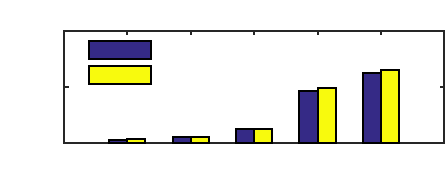
\includegraphics[width=\unitlength]{numberofframessvg.pdf}}%
    \put(0.49756185,0.01128552){\makebox(0,0)[lb]{\smash{\small{t[s]}}}}%
    \put(0.09282368,0.08132461){\makebox(0,0)[lb]{\smash{0}}}%
    \put(0.06443245,0.20731075){\makebox(0,0)[lb]{\smash{50}}}%
    \put(0.03604122,0.33329678){\makebox(0,0)[lb]{\smash{100}}}%
    \put(0.35378421,0.29015447){\makebox(0,0)[lb]{\smash{kinect}}}%
    \put(0.35378421,0.23448302){\makebox(0,0)[lb]{\smash{ensenso}}}%
    \put(0.27065576,0.05747682){\makebox(0,0)[lb]{\smash{1}}}%
    \put(0.41567291,0.05916184){\makebox(0,0)[lb]{\smash{6}}}%
    \put(0.55919591,0.06036764){\makebox(0,0)[lb]{\smash{9}}}%
    \put(0.69462102,0.05909079){\makebox(0,0)[lb]{\smash{25}}}%
    \put(0.83415963,0.05814475){\makebox(0,0)[lb]{\smash{30}}}%
    \put(0.02193696,0.08258763){\rotatebox{90}{\makebox(0,0)[lb]{\smash{\small{Number of frames}}}}}%
  \end{picture}%
\endgroup%

\caption{Number of frames used to model the 'toy car' (object see in Fig.~ \ref{fig:test_objects}). The time stamp of each bar corresponds to that of modelling result in Fig.~\ref{fig:time_evolution}.}
\label{fig:numberofframes}
\end{figure}

\subsubsection{Parameter tuning}
We choose the bunny object to tune the parameter of weights in Equ.~\ref{equ:weights}, because the surface distribution of this object is relative complex. The intuition behind this is if we have a good evaluation model for a complex object, the model should also be able to generalize for simple objects.  Totally we need to determine four weights to evaluate a grasp. Since the sum of all the weights equals one, we only need to tune three of them. In order to compare the effect of each weight, we set one of them to one and the others to zero. Then we use the search algorithm to compute the best grasp configuration. Fig.~\ref{fig:weights1} depicts the best grasp we obtain if we only use the first criterion (Non-zero contact angle). The desired grasp position is on one ear of the bunny. The contact normals are almost anti-parallel to each other. However, it is obviously not an optimal grasp. In Fig.~\ref{fig:weights2}, only the second criterion (Non-optimal finger placement) is activated, the contacts of the best grasp are on the front and the back of the bunny. The contact normals are however not parallel to each other, which may lead to grasp slippage in reality. In Fig.\ref{fig:weights3}, only the third criterion (Distance to center of gravity) is used. The connection line between the contacts passes through the center of gravity, however, the contact normals are not optimal. In Fig.\ref{fig:weights4}, only the fourth criterion (Surface uncertainty) takes effect. During the model reconstruction phase, the back of the bunny is visible to many viewing angles. So the best-desired contact points are on the back of the bunny, where the surface has the lowest uncertainty. However, force closure condition of this grasp is not fulfilled. Based on the analysis, the first criterion has a dominant effect which should be given a larger weight to achieve force closure and a good contact condition. But if the $w_1$ is chosen too large, the best grasp may appear at the side of an object. We need to increase $w_3$ to penalize this effect. $w_2$ and $w_4$ should be chosen as the secondary criterion to motivate more symmetrical contact points as well as making contacts on the surface with low uncertainty. Finally, we find $w_1= 0.6$, $w_2 = w_4 = 0.1$ and $w_3 = 0.2$ are a good trade-off between the four criteria. In the experiment, we use the same parameter to evaluate grasps on other objects. Although the shape of other objects is way different from the bunny object, the experimental result verifies that the chosen parameters also perform well for these objects.

\begin{figure}[!htb]
    \centering
    \begin{subfigure}[b]{0.45\textwidth}
        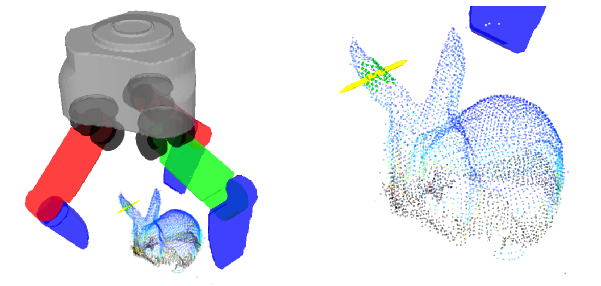
\includegraphics[width=\textwidth]{weights1.png}
        \caption{\textit{Non-zero contact angle} ($w_1 = 1$, $w_2=w_3=w_4=0$)}
        \label{fig:weights1}
    \end{subfigure}
    ~ %add desired spacing between images, e. g. ~, \quad, \qquad, \hfill etc. 
      %(or a blank line to force the subfigure onto a new line)
    \begin{subfigure}[b]{0.45\textwidth}
        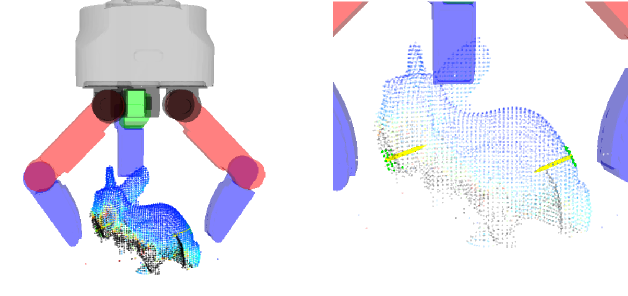
\includegraphics[width=\textwidth]{weights2.png}
        \caption{\textit{Non-optimal finger placement} ($w_2 = 1$, $w_1=w_3=w_4=0$)}
        \label{fig:weights2}
    \end{subfigure}
    ~ %add desired spacing between images, e. g. ~, \quad, \qquad, \hfill etc. 
      %(or a blank line to force the subfigure onto a new line)
    \begin{subfigure}[b]{0.45\textwidth}
        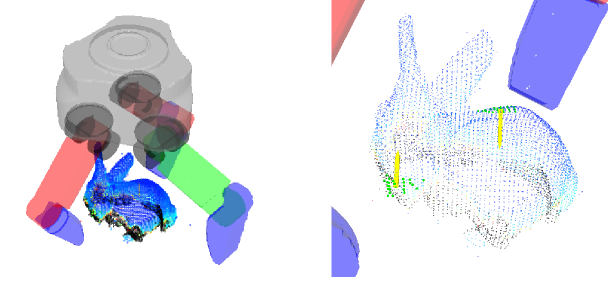
\includegraphics[width=\textwidth]{weights3.png}
        \caption{\textit{Distance to center of gravity} ($w_3 = 1$, $w_1=w_2=w_4=0$)}
        \label{fig:weights3}
    \end{subfigure}
	~
    \begin{subfigure}[b]{0.45\textwidth}
        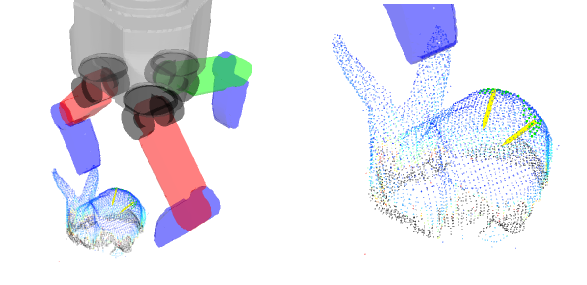
\includegraphics[width=\textwidth]{weights4.png}
        \caption{\textit{Surface uncertainty} ($w_4 = 1$, $w_1 = w_2 = w_3 = 0$)}
        \label{fig:weights4}
    \end{subfigure}
    \caption{The best grasp configuration found by the search algorthm when only one of the four critera is activated. Green points indicate the contact regions. The yellow lines show the normal lines of each contact region.}\label{fig:weights_evaluation}
\end{figure}

\subsection{Performance evaluation on grasp synthesis algorithm}
To generate a viable grasp we first fit a bounding box to a point cloud that is segmented from the table. Based on the estimate of the bounding box, we compute for each object an initial pinch grasp, which is aligned to the bounding box. The initial grasp is used
to initialize the grasp synthesis algorithm. We evaluate the performance of grasp generation in terms of the number of samples. Fig.~\ref{fig:algo_runtime} depicts the time consumption to compute a grasp with a  different number of samples. The computation time increases linearly with the number of grasp samples. We get the variance of time consumption by running the algorithm 10 times for a fixed number of samples. By evaluating the algorithm on three different objects, we also show that the computation time is not correlated with the object type. Fig.~\ref{fig:algo_prob} illustrates the maximum success probability to the number of samples. The maximum success probability can be found after evaluating approximate 200 samples, which means our algorithm can find a viable grasp within 2 seconds. Comparing the speed of a similar work~\cite{Mahler2015}, which also uses signed distance function to model objects, our algorithm is at least 30 times faster.

\begin{figure}[!htpb]
\centering
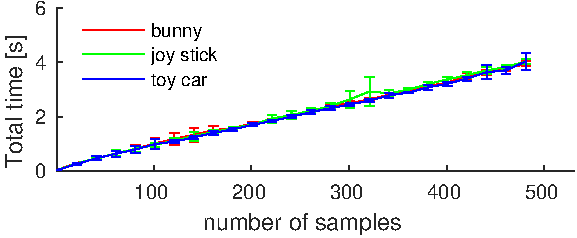
\includegraphics[width=0.7\linewidth]{figure/algo_runtime2-crop.pdf}
\caption{The mean computation time of the grasp generation algorithm scales linearly with the number of samples. The variance is computed by evaluating 10 times for a given number of samples.}
\label{fig:algo_runtime}
\end{figure}


\begin{figure}[!htpb]
\centering
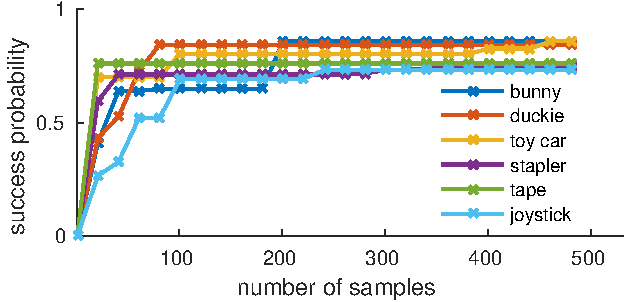
\includegraphics[width=0.7\linewidth]{figure/algo_prob2-crop.pdf}
\caption{The algorithm converges approximately by evaluating 200 samples.}
\label{fig:algo_prob}
\end{figure}


\subsection{Performance on grasping accuracy}
In our experiments, we define three types of outcomes to judge a grasping attempt. They are success with precision (S.w.P),  success (S.) and failure (F). S.w.P means the object is successfully picked up and placed back while the gripper does not displace the object more than 1 cm or more than 30 degrees during force closure. An outcome is marked as S., when the object is successfully picked up in spite of being displaced or rotates within the gripper. An attempt is marked as failure if the object is not successfully picked up or slips out of the gripper. 

Table \ref{tab:result} summarizes the result for a total number of 200 grasping attempts. Our algorithm has achieved 93.5\% success rate of lifting the objects and 79.5 \%  success rate of grasping with precision. The robot manages to grasp 'duckie' and 'correction fluid' without failure. 7 objects are successfully grasped with only a single failure. Fig.~\ref{fig:grasp_example} illustrates some successful grasps generated from our algorithm. 

Among all the objects we used in the experiments, `PS3 Joystick' is the most difficult object for the robot to pick up. Depending on the viewing angle, the hand-mounted Ensenso stereo camera sometimes does not provide reliable depth images so that the object model is only partially integrated or the integration contains large uncertainty. Noted that there are only a few viable pinch grasps which can be used to lift the `PS3 Joystick'. These viable grasps are all located in the middle. When the contact regions for these viable grasps are not well modeled or have large uncertainty, our algorithm is not capable of finding them. These phenomena are also observed for the `screw driver' and the `stapler'. For these two objects, the region where the surface is black results in a large uncertainty in the model. Since these objects contain more feasible grasps, our robot still manages to pick up them successfully. However, the robot has a lower success rate on these objects if S.w.P criterion is used to assess the grasp outcome. Fig.~\ref{fig:slip_staple} depicts one common grasp generated from our algorithm for the `stapler'. Our algorithm tends to find grasps at the end side  of the `stapler', because that region are well modeled and certain to the robot. Since this grasp cannot counteract the wrench generated by the gravity, as soon as the object is lifted up, an in-gripper  object rotation may happen.   

\begin{figure}[!htpb]
\centering
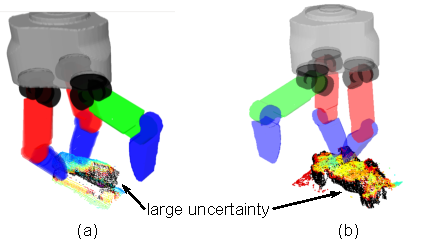
\includegraphics[width=0.7\linewidth]{figure/non_optimal_grasp.pdf}
\caption{(a) A grasp generated by our algorithm for the 'stapler'. Our algorithm tends to generate grasp in the region where the uncertainty is small, which leads to an non-optimal grasp for this case. This grasp may lead to an in-gripper rotation, because it cannot counteract the wrench of gravity. (b) The black points indicate that the side surface of the object has a large uncertainty, however these regions are the only good contact region for a stable grasp. Since our algorithm avoids to generate grasps on uncertainty surfaces, an non-stable grasp is found at one control axis of the `PS3 Joystick'.}
\label{fig:slip_staple} 
\end{figure}

\begin{figure*}[!htpb]
\centering
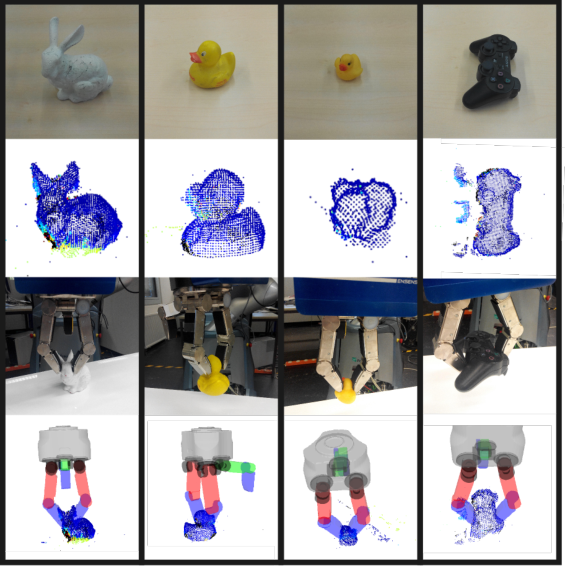
\includegraphics[width=0.8\linewidth]{figure/successful_grasps_illustration.pdf}
\caption{Grasps generated by the algorithm with successful execution.}
\label{fig:grasp_example} 
\end{figure*}

\begin{figure*}[!htpb]
\centering
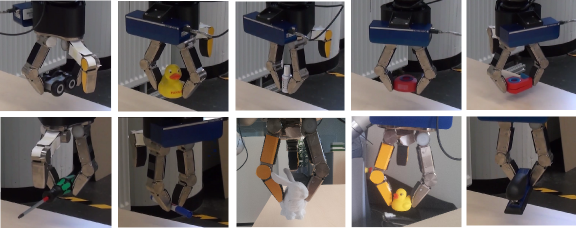
\includegraphics[width=0.8\linewidth]{figure/success_grasp_real.png}
\caption{Successful grasps executed by the robot. }
\label{fig:success_grasps}
\end{figure*}



\begin{table}[!htpb]
\centering
\begin{tabular}{lrrr}
Object           & \multicolumn{1}{c}{S.} & \multicolumn{1}{c}{F.} & \multicolumn{1}{c}{S.w.P} \\
Bunny            & 19/20                  & 1/20                   & 15/20                     \\
Big duck         & 19/20                  & 1/20                   & 16/20                     \\
Tape rectangular & 19/20                  & 1/20                   & 19/20                     \\
Tape triangle    & 19/20                  & 1/20                   & 19/20                     \\
Stapler          & 19/20                  & 1/20                   & 14/20                     \\
Toy car          & 19/20                  & 1/20                   & 18/20                     \\
Duckie           & 20/20                  & 0/20                   & 20/20                     \\
Screwdrawer      & 19/20                  & 1/20                   & 11/20                     \\
PS3 Joystick     & 14/20                  & 6/20                   & 7/20                      \\
Correction fluid & 20/20                  & 0/20                   & 20/20                     \\
Summary          & \textbf{93.5\%}        & 6.5\%            & \textbf{79.5\%}                  
\end{tabular}
\caption{(S. = success, F. = failure, S.w.P = Success with precision). Experimental result for a total of 200 grasping attempts. An outcome is classified as S.w.P when gripper successfully picked the object without displacing the object more than 1 cm or 30 degree. This criterion is strict comparing to a standard way to access grasping success.} 
\label{tab:result}
\end{table}

\subsection{Comparison with one baseline approach}
We choose the approach proposed by Fischinger et al. \cite{FischingerWV15} as the baseline  for comparison. This method calculates grasps from a given point cloud using a so-called `\textit{Height Accumulated Features}'(HAF). It has been shown that the approach was adapted to different robots and gripper systems for grasping a variety of unknown objects. In order to use their approach for grasping with our system, we need to adapt the calculated grasping points to our gripper. We use the implementation from \url{http://wiki.ros.org/haf_grasping} in our experiments. The default parameters are used to calculate the grasping points. The output of the method is 2D positions of two grasp points. Additionally, a grasp realization step is required to compute the height of a grasp for executing a real grasp. They implement the grasp realization step in OpenRAVE simulator, in which a  mesh of an object is calculated for collision checking. Then they use a heuristic to compute a real grasp: setting a manipulator about 7 cm away from the object. As this implementation is not available for our system, we implement a realization step by setting the height of the grasping points at the middle of an object's bounding box.  

Fig.~\ref{fig:baseline_comparison} depicts a grasp calculated by HAF and our approach on the bunny object. The grasp calculated by HAF may lead to a grasp failure since the region of contact points lies around the head of the bunny. In these regions, there is no flat surface to establish a stable contact. On the contrary, the best grasp calculated by our method is on the body of the bunny. This is more likely to succeed than the one calculated by HAF.  
\begin{figure}[!htb]
    \centering
    \begin{subfigure}[t]{0.45\textwidth}
        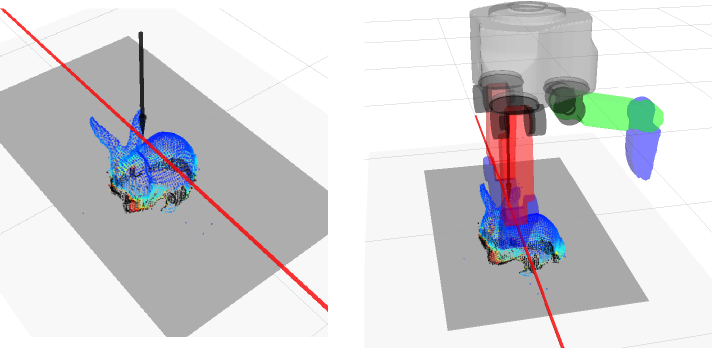
\includegraphics[width=\textwidth]{haf_grasp.png}
        \caption{Left: the best grasp point calculated by the baseline approach. The red line indicates the close direction. The black arrowed line shows the approach direction and the position of a gripper. Right: grasp realization for our gripper.}
        \label{fig:haf_grasp}
    \end{subfigure}
    ~ %add desired spacing between images, e. g. ~, \quad, \qquad, \hfill etc. 
      %(or a blank line to force the subfigure onto a new line)
    \begin{subfigure}[t]{0.45\textwidth}
        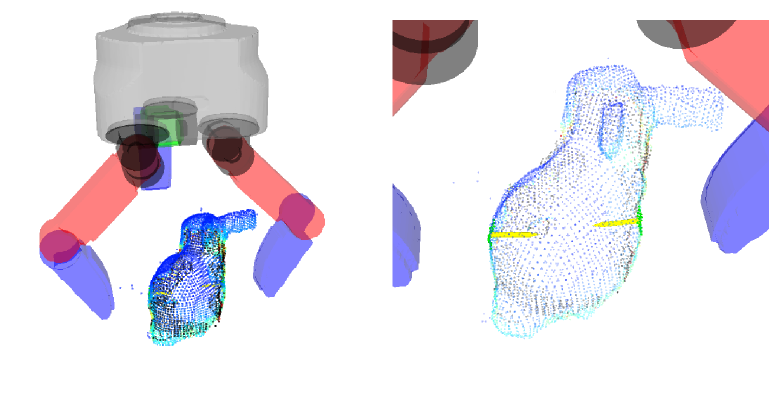
\includegraphics[width=\textwidth]{best_grasp.png}
        \caption{Left: the best grasp calculated by our method with weights ($w_1 = 0.6, w_3=0.2, w_2=w_4=0.1$). Right: A zoom-in visualization of the contact points.  }
        \label{fig:best_grasp}
    \end{subfigure}
    \caption{A comparison of a grasp calculated by the baseline method and our method. The grasp generated by the baseline approach may lead to grasping slippage due to sub-optimal contacts. }\label{fig:baseline_comparison}
\end{figure}

In order to systematically compare both approaches, we conduct the same real grasp experiment on the test object set with HAF. We only use the hand-mounted stereo camera to obtain an input point cloud for HAF as the stereo camera provides more precise data than the Kinect. The input point cloud represents a top view of a test object. The experiment result is summarized in Tab.~\ref{tab:baseline_compare}. 
We exclude the object `duckie' and `Correction fluid' from the comparison because the point cloud which represents them can not be robustly segmented during the experiment. Due to the segmentation error, a lot of grasp failure occurs for these two objects when using the baseline method. 

In summary, our method achieves a lower error rate than HAF based on 320 grasp trials in total. HAF can perform well on small regular objects, while has difficulty to grasp objects with a complex surface distribution like `Bunny'. HAF also not performs well on `stapler' or `screw driver'. One reason of failure for these two objects is that the input point cloud sometimes only contains a partial view of the object. The material of the objects may cause reflections, e.g. the input point cloud may not contain the shaft side of the `screw driver', which may cause the calculated grasp being too far from the center of mass. Both approaches have difficulty in grasping `PS3 joystick'. The reason for that has been discussed previously.
\begin{table}[!htb]
\centering
\begin{tabular}{lrr}
               & Our method & HAF   \\
Bunny          & 19/20      & 16/20 \\
Big duck       & 19/20      & 18/20 \\
Tape rec.      & 19/20      & 19/20 \\
Tape triang.   & 19/20      & 20/20 \\
Stapler        & 19/20      & 12/20 \\
Toy car        & 19/20      & 20/20 \\
Screwdrawer    & 19/20      & 7/20  \\
PS3 Joystick   & 14/20      & 13/20 \\
Nr. of failure & \textbf{13}         & \textbf{35}   
\end{tabular}
\caption{Successful grasp executed by HAF (baseline method) and our method on a subset of the test objects. Our method achieves a lower error rate than the baseline method.}
\label{tab:baseline_compare}
\end{table}


\subsection{Discussion} 
Precise grasping is one of the advantages of the proposed approach. By explicitly modeling the surface geometry and its uncertainty, we can compute grasps with more precision so that during force closure the object is less probable to be displaced. Due to the unknown dynamics of the object, displacement of the object may result in grasp failure more likely, when an unexpected situation such as slipping happens.

Most approaches address the problem of grasping an  unknown object by finding grasp relevant feature from a single measurement. Single measurement, however, may contain large uncertainty. Partial and occlusion of the measurement usually result in a hard situation for grasp detection. Well defined grasp features such as surface normals can not be used because the region where contacts take place are usually not observable from a single measurement. Our approach handles this problem by integrating multiple measurements so that we can use well-defined features, namely, the surface normals and the modeling uncertainty to assess the viability of grasps. 

Recently, some approach exploits deep learning for grasp classification~\cite{Pinto2015}, however gathering training examples require enormous effort. The training data is gathered by running a robot over 700 hours. In addition, the training examples are basically images with a labeled grasp. The learned model may not be able to generalize to another environment with a different lighting condition. Our approach does not require any training data, and still gets a competitive result. The result indicates that for grasping problem  choosing of a suitable representation can improve the system performance dramatically. 

There are also some limitations in the current approach. As our approach requires a pre-segmentation of the  object, applying this  method to a cluttered scenario where lots of objects stacked to each other relies on a sophisticated segmentation algorithm. These algorithms may not be available at the moment. In addition, our approach can not handle transparent objects such as `glasses', `coins', `small screws'. In these cases, exploiting other sensing modality such as a color camera may help. Another drawback of our approach is that the robot is required to observe the objects with different pre-defined view angles prior to grasping, this may increase the time of task execution. Regarding this problem, one may exploit active perception approaches to minimize the travel distance while still acquiring sufficient information for a stable grasp. 

\section{Summary}
In this chapter, we present a probabilistic approach to address the problem of grasp synthesis for unknown objects. Our method explicitly models the uncertainty for the items which are presented to the robot for the first time. Our method finds the most promising grasp configuration which maximizes the grasp success probability. We especially choose challenging novel objects in our grasping experiment. The results demonstrate that our approach is capable of grasping a range of novel while unknown objects precisely and outperform a state-of-the-art method.

One of the important aspects of the proposed approach is that without the benefit of learning, our system still achieves a good perform in experiments, which may indicate that the choice of object representation and the model of grasp evaluation play a significant role for grasping. Our intuition behind this is that learning from large scale experiments introduces semantics and high-level information for the choice of grasps, while for low-level precision grasping we still need a suitable object representation to handle uncertainty and achieve robustness. One direction of the future work is to combining other sensor modalities such as RGB information into the current approach so that we can benefit from
 the result of large scale learning to reinforce the approach with semantics and task level information. Another direction of the future work can be exploiting the environment constraints explicitly to allow contact-rich grasping even in crowded environments.




